\RequirePackage{iftex}
\ifPDFTeX
  \errmessage{This document requires XeLaTeX or LuaLaTeX. Please change your compiler.}
\fi
\documentclass[12pt]{report}

% @@@@@@@@@@@@@@@@@@@@@@@@@@@@@@@@@@@@@@@@@@@@@@@@@@@@@@@@@@@@>
% VALORES A MODIFICAR POR USTED:
% @@@@@@@@@@@@@@@@@@@@@@@@@@@@@@@@@@@@@@@@@@@@@@@@@@@@@@@@@@@@>

% NOTE: Leer nota en el README sobre la font.

\newcommand{\titulo}{Desarrollo de un pipeline basado en DRAFTS para detección y clasificación de transientes de radio con adaptación y extensión en regímenes de alta frecuencia}
\newcommand{\ciudad}{Valparaíso} % e.g. Valparaíso
% TODO: Consultar el formato de los nombres:
\newcommand{\nombrealumno}{Sebastian Salgado Polanco}
\newcommand{\nombreprofesor}{Daniela Opitz}
\newcommand{\nombrecorreferente}{Marylin Cruces}
% Mes y año del examen
\newcommand{\mesexamen}{Enero}
\newcommand{\anioexamen}{2025}
% Dedicatoria y agradecimientos
\newcommand{\dedicatoria}{
Considerando lo importancia de este trabajo para los alumnos, este apartado es para que el autor entregue palabras personales para dedicar este documento. La extensión puede ser de máximo una hoja y se deben mantener este formato, tipo y tamaño de letra.
}
\newcommand{\agradecimientos}{
Considerando la importancia de este trabajo para los alumnos, este apartado se podrá incluir en el caso de que el autor desee agradecer a las personas que facilitaron alguna ayuda relevante en su trabajo para la realización de este documento. La extensión puede ser de máximo una hoja y se deben mantener este formato, tipo y tamaño de letra.
}
\newcommand{\resumen}{
El resumen y las palabras clave no deben superar la mitad de la página, donde debe precisarse brevemente: 1) lo que el autor ha hecho, 2) cómo lo hizo (sólo si es importante detallarlo), 3) los resultados principales, 4) la relevancia de los resultados. El resumen es una representación abreviada, pero comprensiva de la memoria y debe informar sobre el objetivo, la metodología y los resultados del trabajo realizado.
}
\newcommand{\resumeningles}{
Corresponde a la traducción al idioma inglés del Resumen anterior. Sujeto a la misma regla de extensión del Resumen.
}
\newcommand{\palabrasclave}{
Cinco es el máximo de palabras clave para describir los temas tratados en la memoria, ponerlas separadas por punto y comas.
}
\newcommand{\palabrasclaveingles}{
Corresponde a la traducción al idioma inglés de Palabras Clave anteriores.
}
% @@@@@@@@@@@@@@@@@@@@@@@@@@@@@@@@@@@@@@@@@@@@@@@@@@@@@@@@@@@@>

% Paquete para importar imágenes
\usepackage{graphicx}
% Directorio de las imágenes
\graphicspath{ {figures/} }

% Idioma y fuentes
\usepackage[spanish,es-tabla]{babel}
\usepackage[T1]{fontenc}

\usepackage{fontspec}
% Selección robusta de fuente principal con respaldo en Windows
\newcommand{\MainFontName}{Carlito}
\IfFontExistsTF{Carlito}{
  \renewcommand{\MainFontName}{Carlito}
}{
  \IfFontExistsTF{Calibri}{
    \renewcommand{\MainFontName}{Calibri}
  }{
    \renewcommand{\MainFontName}{Latin Modern Roman}
  }
}
\setmainfont{\MainFontName}[BoldFont={* Bold}, ItalicFont={* Italic}]

% Paquete para definir cualquier tamaño de font
\usepackage{anyfontsize}

% Tamaño de la página y márgenes
\usepackage[letterpaper,top=2.5cm,bottom=3cm,left=3cm,right=3cm,marginparwidth=1.75cm]{geometry}

% Determinar interlineado:
\renewcommand{\baselinestretch}{1.0}

% Eliminar sangrías:
\setlength{\parindent}{0cm}

% Paquete para definir los formatos de los títulos
\usepackage[explicit]{titlesec}

\titleformat{name=\section}[block]{\fontsize{16}{24}\selectfont\bfseries}{}{0pt}{#1}
\titleformat{name=\section,numberless}[block]{\fontsize{16}{24}\selectfont\bfseries}{}{0pt}{#1}
\titlespacing*{name=\section}{0pt}{0pt}{0.5cm}
\titlespacing*{name=\section,numberless}{0pt}{0pt}{0.5cm}

% Formato para subsecciones numeradas
\titleformat{name=\subsection}[block]{\fontsize{14.4}{18}\selectfont\bfseries}{\arabic{mychapter}.\arabic{subsection}}{0.5em}{#1}
\titlespacing*{name=\subsection}{0pt}{0pt}{0.3cm}

% Formato para subsubsecciones numeradas
\titleformat{name=\subsubsection}[block]{\fontsize{12.96}{16}\selectfont\bfseries}{\arabic{mychapter}.\arabic{subsection}.\arabic{subsubsection}}{0.5em}{#1}
\titlespacing*{name=\subsubsection}{0pt}{0pt}{0.2cm}

% Separación entre parrafos
\setlength{\parskip}{0.4cm}

% Paquetes de utilidad general
\usepackage{amsmath}
\usepackage{graphicx}
\usepackage{float}
\usepackage{booktabs}  % Para comandos de tablas profesionales (\toprule, \midrule, \bottomrule)
\usepackage[table]{xcolor}  % Para colorear filas y columnas en tablas
\usepackage{tikz}       % Para diagramas y gráficos
\usetikzlibrary{positioning,shapes.geometric,arrows.meta}
\usepackage{algorithm}  % Para pseudocódigos
\usepackage{algpseudocode}  % Para pseudocódigos con estilo
\usepackage{listings}   % Para código con formato
\usepackage[colorlinks=true, allcolors=blue]{hyperref}

% Formato de las tablas de contenido
\usepackage{tocbasic}

%% Originalmente se usaba tocstyle en vez de tocbasic.
%% Si se quiere usar, descomentar:
% \usepackage[tocflat]{tocstyle}
% \usetocstyle{allwithdot}
%% tocstyle.sty se obtener de https://github.com/firemodels/fds/blob/master/Manuals/LaTeX_Style_Files/tocstyle.sty

% Para obtener el número de la última página
\usepackage{lastpage}

% Header y footer
\usepackage{fancyhdr}
\fancypagestyle{portada}{
    \lhead{}
    \chead{}
    \rhead{}
    \lfoot{}
    \cfoot{\fontsize{10}{12}\selectfont \thepage}
    \rfoot{}
    \renewcommand{\headrulewidth}{0pt}
}
\fancypagestyle{intermedio}{
    \lhead{}
    \chead{\fontsize{10}{12}\selectfont\MakeUppercase{\titulo}}
    \rhead{}
    \lfoot{}
    \cfoot{\fontsize{10}{12}\selectfont Página \textbf{\thepage}\ de \textbf{\pageref{LastPage}}}
    \AtEndDocument{\label{LastPage}}
    \rfoot{}
    \renewcommand{\headrulewidth}{1pt}
}

% Numeración de secciones hasta subsubsecciones
\setcounter{secnumdepth}{3}  % Numerar hasta subsubsecciones
\setcounter{tocdepth}{3}     % Incluir subsubsecciones en tabla de contenidos

% Comandos para secciones
\newcounter{mychapter}
\setcounter{mychapter}{0}
\setcounter{section}{0}
\setcounter{figure}{0}
\setcounter{table}{0}
\newcommand{\secnumbersection}[1]{
\stepcounter{mychapter}
\stepcounter{section}
\phantomsection
\section*{CAPÍTULO \themychapter \texorpdfstring{\\}\ #1}
\addcontentsline{toc}{section}{CAPÍTULO \themychapter : #1}
\setcounter{subsection}{0}
\setcounter{figure}{0}
\setcounter{table}{0}
\renewcommand{\thesubsection}{\arabic{mychapter}.\arabic{subsection}}
}
\newcommand{\secnumberlesssection}[1]{
\section*{#1}
\phantomsection
\addcontentsline{toc}{section}{#1}
\setcounter{subsection}{0}
}

% Nombres
\addto\captionsspanish{\renewcommand{\contentsname}{ÍNDICE DE CONTENIDOS}}
\addto\captionsspanish{\renewcommand{\listfigurename}{ÍNDICE DE FIGURAS}}
\addto\captionsspanish{\renewcommand{\listtablename}{ÍNDICE DE TABLAS}}
\makeatletter
\renewenvironment{thebibliography}[1]
     {\secnumberlesssection{REFERENCIAS BIBLIOGRÁFICAS}
      \@mkboth{\MakeUppercase\bibname}{\MakeUppercase\bibname}%
      \list{\@biblabel{\@arabic\c@enumiv}}%
           {\settowidth\labelwidth{\@biblabel{#1}}%
            \leftmargin\labelwidth
            \advance\leftmargin\labelsep
            \@openbib@code
            \usecounter{enumiv}%
            \let\p@enumiv\@empty
            \renewcommand\theenumiv{\@arabic\c@enumiv}}%
      \sloppy
      \clubpenalty4000
      \@clubpenalty \clubpenalty
      \widowpenalty4000%
      \sfcode`\.\@m}
     {\def\@noitemerr
       {\@latex@warning{Empty `thebibliography' environment}}%
      \endlist}
\makeatother

% Configuración de numeración de figuras y tablas
\renewcommand{\thefigure}{\arabic{mychapter}.\arabic{figure}}
\renewcommand{\thetable}{\arabic{mychapter}.\arabic{table}}

% Configuración para pseudocódigos con estilo profesional
\algnewcommand\algorithmicinput{\textbf{Entrada:}}
\algnewcommand\algorithmicoutput{\textbf{Salida:}}
\algnewcommand\Input{\item[\algorithmicinput]}
\algnewcommand\Output{\item[\algorithmicoutput]}

% Configuración de listings para código
\lstset{
    basicstyle=\ttfamily\small,
    keywordstyle=\bfseries,
    commentstyle=\itshape,
    stringstyle=\itshape,
    numbers=left,
    numberstyle=\tiny,
    stepnumber=1,
    numbersep=5pt,
    frame=single,
    breaklines=true,
    breakatwhitespace=true,
    tabsize=2,
    showstringspaces=false
}

% Personalizar Tabla de Contenidos

\usepackage{tocloft}
\renewcommand{\cftsecfont}{\fontsize{12}{14}\selectfont\fontspec{\MainFontName}}
\renewcommand{\cftsubsecfont}{\fontsize{12}{14}\selectfont\fontspec{\MainFontName}}
\renewcommand{\cftsubsubsecfont}{\fontsize{12}{14}\selectfont\fontspec{\MainFontName}}

\renewcommand\cftfigfont{\fontsize{12}{14}\selectfont\fontspec{\MainFontName}}

% Links sin color
\usepackage{hyperref}
\hypersetup{colorlinks = false}

% Comando para secciónes sin enumeración
% (sugerido por @anibalbastiass https://github.com/autopawn/tex-thesis-template/issues/5#issuecomment-916106128)
\newcommand{\secnumberlesssubsection}[1]{
\subsection*{#1}
\phantomsection
\addcontentsline{toc}{subsection}{#1}
\setcounter{subsection}{0}
}
% Forma de uso:
% \secnumberlesssubsection{"Sub seccion sin enumeración"}

% @@@@@@@@@@@@@@@@@@@@@@@@@@@@@@@@@@@@@@@@@@@@@@@@@@@@@@@@@@@@>
\begin{document}
\sloppy % Para evitar que referencias se escapen de los márgenes.

\pagestyle{portada}
\pagenumbering{roman}
% NOTE: Este archivo contiene la portada, la dedicatoria, los agradecimientos y el resumen.
% __NO ES NECESARIO MODIFICAR ESTE ARCHIVO__, esas se modifican con los comandos que aparecen en main.tex
%@@@@@@@@@@@@@@@@@@@@@@@@@@@@@@@@@@@@@@@@@@@@@@@@@@@@@@@@@@@@@@
\begin{titlepage}
\begin{center}
\noindent
{\fontsize{18}{22}\selectfont UNIVERSIDAD TÉCNICA FEDERICO SANTA MARÍA \\}
{\fontsize{16}{19}\selectfont DEPARTAMENTO DE INFORMÁTICA \\}
{\fontsize{16}{19}\selectfont \MakeUppercase{\ciudad}\ - CHILE \\}
\vspace{1.5cm}

\includegraphics[width=4.41cm,height=3.34cm]{logo/logo.jpg} \\
\vspace{1.5cm}
{\fontsize{20}{24}\selectfont ``\MakeUppercase{\titulo}'' \\}
\vfill
{\fontsize{16}{19}\selectfont \MakeUppercase{\nombrealumno} \\}
\vfill
{\fontsize{16}{19}\selectfont MEMORIA PARA OPTAR AL TÍTULO DE \\}
{\fontsize{16}{19}\selectfont INGENIERO CIVIL EN INFORMÁTICA \\}
\vspace{1.5cm}
{\fontsize{14}{17}\selectfont Profesor Guía: \nombreprofesor \\}
{\fontsize{14}{17}\selectfont Profesor Correferente: \nombrecorreferente \\}
\vspace{2.5cm}
{\fontsize{14}{17}\selectfont \mesexamen\ - \anioexamen \\}
\end{center}
\end{titlepage}

%@@@@@@@@@@@@@@@@@@@@@@@@@@@@@@@@@@@@@@@@@@@@@@@@@@@@@@@@@@@@@@
\newpage
\setcounter{page}{2}
\
\vfill
\vfill
\begin{flushright}
\noindent {\fontsize{16}{19}\selectfont \textbf{DEDICATORIA} \\}
\end{flushright}
\begin{flushright}
\noindent \dedicatoria
\end{flushright}
\vfill
%@@@@@@@@@@@@@@@@@@@@@@@@@@@@@@@@@@@@@@@@@@@@@@@@@@@@@@@@@@@@@@
\newpage
\begin{center}
\noindent {\fontsize{16}{19}\selectfont \textbf{AGRADECIMIENTOS} \\}
\end{center}
\noindent \agradecimientos
\vfill
%@@@@@@@@@@@@@@@@@@@@@@@@@@@@@@@@@@@@@@@@@@@@@@@@@@@@@@@@@@@@@@
\newpage
\secnumberlesssection{RESUMEN}
\vspace{0.3cm}
\noindent \textbf{Resumen---}\resumen \ \\
\vspace{0.3cm} \\
\noindent \textbf{Palabras Clave---}\palabrasclave \ \\
% @@@@@
\vspace{1.2cm} \\
% @@@@@
%\noindent {\fontsize{16}{19}\selectfont \textbf{ABSTRACT}}
%\vspace{1.2cm} \\
\secnumberlesssection{ABSTRACT}
\vspace{0.3cm}
\noindent \textbf{\emph{Abstract}---}\resumeningles \ \\
\vspace{0.3cm} \\
\noindent \textbf{\emph{Keywords}---}\palabrasclaveingles \ \\
%@@@@@@@@@@@@@@@@@@@@@@@@@@@@@@@@@@@@@@@@@@@@@@@@@@@@@@@@@@@@@@


\newpage
\secnumberlesssection{GLOSARIO}

{\setlength{\parskip}{0cm} % Evita saltos extra entre elementos.

ALMA: \textit{Atacama Large Millimeter/submillimeter Array}. Interferómetro de 66 antenas operando en 0.32–3.6\,mm; en modo \textit{phased} suma coherentemente su área efectiva para funcionar como un “plato” único de gran diámetro. \citep{veracasanova2025}

AMBER: \textit{A Modular GPU-Based Real-time} pipeline para búsqueda de pulsos individuales y transientes rápidos. \citep{Sclocco_2020_AMBER}

APS: \textit{ALMA Phased Sum} (ALMA en modo \textit{phased}). Suma coherente de señales que permite \textit{baseband} y VLBI.

Baseband: Voltajes complejos sin detectar (\textit{raw complex voltages}) alrededor del evento, útiles para reprocesado fino y localización interferométrica.

Boxcar: Filtro promediador rectangular usado en \textit{matched filtering} para cubrir anchos de pulso diversos. \citep{Rajwade_2024_Review}

CenterNet: Detector de objetos que representa objetos como centros (picos) en mapas de calor; usado en DRAFTS para detectar la firma en el plano tiempo–DM. \citep{Zhou_2019_CenterNet}

CHIME/FRB: Backend de FRBs del radiotelescopio CHIME; produce catálogos uniformes y, con \textit{Outriggers}, localizaciones precisas. \citep{CHIMEFRB_2021_Catalog1,CHIME_Outriggers_Overview}

CNN: \textit{Convolutional Neural Network}. Arquitecturas profundas para clasificación de candidatos FRB vs.\ RFI. \citep{Agarwal_2020}

DADA / PSRDADA: \textit{Distributed Acquisition and Data Analysis}. Formato y \textit{ring buffers} en memoria compartida para adquisición/flujo de datos en tiempo real. \citep{PSRDADA_ascl,DSPSR_DADA_Header}

DD: \textit{Dedispersión}. Corrección del retardo por plasma ($\propto \nu^{-2}$) para concentrar la señal al DM óptimo; puede ser incoherente (tiempo) o en dominio de Fourier. \citep{Rajwade_2024_Review}

DRAFTS: \textit{Deep learning-based Radio Fast Transient Search}. Pipeline que integra dedispersión acelerada, detección (CenterNet) y clasificación (ResNet) en un flujo unificado. \citep{zhang2024drafts}

DRAFTS++: Extensión modular de DRAFTS propuesta en esta memoria: I/O estandarizado, dedispersión acelerada, \textit{chunking}, clasificación y rutas especializadas mm, con \textit{logging} y \textit{alerting}.

EVN: \textit{European VLBI Network}. Red VLBI para localización de alta precisión en radio.

FDMT: \textit{Fast Dispersion Measure Transform}. Algoritmo óptimo en sensibilidad con menor complejidad que \textit{brute force} para dedispersión incoherente. \citep{Zackay_2014_FDMT}

FDD: \textit{Fourier-Domain Dedispersion}. Implementa los retardos como rotaciones de fase en el dominio de Fourier; computacionalmente afín a GPU cuando se requieren muchos DMs. \citep{Bassa_2021_FDD}

FETCH: Clasificador automatizado basado en \textit{transfer learning} (CNNs) para candidatos de FRB y RFI. \citep{Agarwal_2020}

FITS / PSRFITS: Formato estándar astronómico; PSRFITS es el perfil para pulsar/transientes adoptado por \textsc{PSRCHIVE}. \citep{Hotan_2004_PSRFITS}

FRB: \textit{Fast Radio Burst}. Ráfaga de radio de duración milisegundos, altamente dispersa y de origen extragaláctico. \citep{Petroff_2022,Zhang_2020}

Heimdall: Software de búsqueda de pulsos individuales acelerado en GPU; admite \texttt{SIGPROC filterbank} y \texttt{PSRDADA}. \citep{Heimdall_Use}

IQRM: \textit{Inter-Quartile Range Mitigation}. Enmascaramiento adaptativo de RFI por detección robusta de \textit{outliers} en bloques cortos; apto para \textit{streaming}. \citep{Morello_2021_IQRM}

Matched Filtering: Correlación con una familia de plantillas (p.ej., \textit{boxcars}) y \textit{downsampling} multi-escala para maximizar S/N en distintos anchos. \citep{Rajwade_2024_Review}

Outriggers (CHIME/FRB): Estaciones remotas que permiten localizaciones $\sim$mas–decenas de mas mediante VLBI sin depender de redes tradicionales. \citep{Lanman_2024_Outrigger,CHIME_Outriggers_Overview}

PRESTO: \textit{PulsaR Exploration and Search TOolkit}. Conjunto de herramientas para búsqueda de pulsos periódicos/simples y diagnóstico. \citep{2011ascl.soft07017R}

PSRCHIVE: Conjunto de bibliotecas y aplicaciones para análisis de datos de pulsar/transientes; base de PSRFITS y estándares de polarización/Stokes. \citep{Hotan_2004_PSRFITS}

ResNet: \textit{Residual Network}. CNN profunda (bloques residuales) usada como columna vertebral de clasificación en DRAFTS. \citep{He_2015_ResNet}

RFI: \textit{Radio Frequency Interference}. Contaminación por señales de origen humano/natural que degrada sensibilidad y genera falsos positivos.

RM: \textit{Rotation Measure}. Medida de rotación de Faraday (rad\,m$^{-2}$) que integra densidad electrónica y campo magnético a lo largo de la línea de visión. \citep{Petroff_2022}

S/N (SNR): Relación señal-ruido. Métrica para umbralado de detección y ranking de candidatos.

SIGPROC filterbank: Formato de serie tiempo–frecuencia muy usado en búsquedas de pulsos únicos; ampliamente soportado por herramientas de búsqueda. \citep{Heimdall_Use}

SK: \textit{Spectral Kurtosis}. Estadístico de no-gaussianidad para detección/mitigación de RFI sin degradar la señal astrofísica. \citep{Nita_2010_SK}

VOEvent: Estándar IVOA para describir y distribuir alertas de eventos transitorios (contenido, transporte y red de distribución). \citep{VOEvent_2_0,VOEvent_Transport}

VLBI: \textit{Very Long Baseline Interferometry}. Interferometría con líneas de base continentales que permite localizaciones de sub-arco-segundo a milisegundos de arco.

Zero-DM filter: Sustracción del promedio por canal en la dinámica no dedispersada para atenuar RFI de banda ancha; debe aplicarse con cautela para no suprimir señales de DM baja o muy anchas. \citep{Rajwade_2024_Review}

}


%Índice de contenidos:
\newpage
\thispagestyle{portada}
\tableofcontents

%Índice de figuras:
\newpage
\thispagestyle{portada}
\phantomsection
\addcontentsline{toc}{section}{ÍNDICE DE FIGURAS}
\listoffigures
\phantomsection
\addcontentsline{toc}{section}{ÍNDICE DE TABLAS}
\listoftables

\newpage
\pagestyle{intermedio}
\pagenumbering{arabic}
\secnumbersection{INTRODUCCIÓN}

\section{Contexto y motivación}
En la última década, la radioastronomía ha revelado la existencia de fenómenos transitorios extremadamente breves y energéticos, entre los que destacan las \textit{ráfagas rápidas de radio} (Fast Radio Bursts, FRBs). Las FRBs son pulsos de emisión de radio de duración del orden de milisegundos, generalmente originados a distancias extragalácticas. Su descubrimiento inicial en 2007 marcó un hito por la intensidad y lejanía de estas señales \cite{Lorimer2007}. El estudio de las FRBs es de gran relevancia científica: estas ráfagas pueden utilizarse como trazadores del medio intergaláctico, aportando información sobre la distribución de materia bariónica y sobre campos magnéticos a escalas cosmológicas, además de ofrecer nuevas oportunidades para la cosmología observacional \cite{Petroff_2022}. 

\begin{figure}[h]
\centering
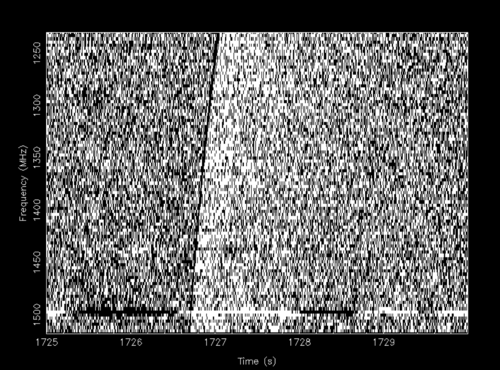
\includegraphics[width=0.8\textwidth]{figures/Lorimer Burst.png}
\caption{Ráfaga de Lorimer: observación de la primera ráfaga de radio rápida detectada, tal como la describió Lorimer en 2006.}
\label{fig:lorimer}
\end{figure}

\section{Problema}
Detectar FRBs en tiempo de procesamiento plantea desafíos considerables. Los radiotelescopios modernos generan volúmenes masivos de datos, lo que dificulta el procesamiento eficiente de observaciones en busca de eventos de milisegundos. A esto se suma la abundante interferencia de radiofrecuencia (RFI) de origen humano, que contamina las señales e imita pulsos astrofísicos, produciendo grandes listas de candidatos falsos. Los métodos tradicionales de búsqueda de pulsos individuales como los algoritmos implementados en suites clásicas tipo PRESTO y Heimdall se basan en dedispersión exhaustiva y umbrales fijos de detección, si bien han sido exitosos, son propensos a listas extensas de falsos positivos y requieren inspección manual intensiva, lo que limita su uso en operación en tiempo (casi) real \cite{CordesMcLaughlin2003, Ransom_2003, Barsdell_2012}. Por otra parte, \textbf{DRAFTS} aporta modelos de detección y clasificación, pero no un pipeline operativo extremo a extremo.

\textbf{TODO (Problema específico)}: Completar con 3–4 frases que describan el vacío exacto en tu contexto (datos disponibles, limitaciones de herramientas actuales en tu entorno, necesidad de near-real-time, etc.).

\section{Objetivos}
\textbf{Objetivo general:} Diseñar e implementar un pipeline basado en DRAFTS para detección y clasificación de transientes de radio, y extenderlo a regímenes de alta frecuencia.\\
\textbf{Objetivos específicos:}
\begin{itemize}
  \item Integrar y operacionalizar los modelos de DRAFTS en un pipeline reproducible.
  \item Diseñar módulos de ingesta, preprocesado, detección, clasificación y reporte.
  \item Adaptar la búsqueda a frecuencias milimétricas (mm-wave) considerando sus particularidades.
  \item Evaluar desempeño (recall, precision, F1, latencia) en banda L y en mm-wave.
\end{itemize}

\textbf{TODO (Medición de objetivos)}: Indicar cómo verificarás cada objetivo (p.ej., latencia \(<\) N s/archivo de 32 GB; F1 \(>\) X en FRB121102).

\section{Preguntas de investigación e hipótesis}
¿Cómo se comporta la detección y clasificación de FRBs al comparar banda L con mm-wave? Hipótesis: la atenuación del patrón bow-tie en mm-wave disminuye sensibilidad de detectores basados en tiempo–DM, mitigable ampliando rango/step de DM y mediante validación por sub-bandas y clasificación a DM\(\approx 0\).

\textbf{TODO (Criterios de falsación)}: Expresar qué resultados refutarían/confirmarían la hipótesis (p.ej., recall relativo mm-wave/L-band, tasa de falsos DM\(\approx\)0).

\section{Principales contribuciones técnicas}
\begin{itemize}
  \item Pipeline DRAFTS-MB con módulos definidos, contratos I/O y configuración.
  \item Estrategias de chunking/slices/overlap con criterios formales de \(\Delta DM\) por smearing.
  \item Integración CenterNet (detección) + ResNet (clasificación) con umbrales robustos (MAD/IQR).
  \item Extensión y validación en mm-wave y lineamientos para operación near-real-time.
\end{itemize}

\textbf{TODO (Evidencias de contribución)}: Enumerar outputs verificables (scripts, configs, artefactos, figuras clave, IDs de commit).

\section{Alcance y limitaciones}
El trabajo se enfoca en búsqueda de pulsos individuales (single-pulse) y no aborda timing ni localización interferométrica plena. Se trabaja con PSRFITS/FIL, con disponibilidad de GPU estándar. Limitaciones incluyen RFI a DM\(\approx 0\), dependencia de metadatos fiables y variabilidad instrumental.

\textbf{TODO (Límites explícitos)}: Añadir supuestos concretos (p.ej., resolución temporal mínima, anchos de banda soportados, formatos exactos, versiones de librerías).

\section{Organización del documento}
Este documento se organiza en diez capítulos más anexos. El Capítulo 2 presenta el marco teórico; el 3, el estado del arte; el 4, los requisitos y el diseño del pipeline; el 5, la implementación; el 6, la metodología experimental y los datasets; el 7, los resultados en banda L; el 8, la extensión a mm-wave (ALMA); el 9, la discusión y amenazas a la validez; y el 10, las conclusiones y trabajo futuro.

\section{Posicionamiento frente a pipelines en tiempo real}
Como motivación y punto de comparación, se discuten arquitecturas operativas de CHIME/FRB, ASKAP/CRAFT y MeerTRAP, destacando diferencias en adquisición, backend, mitigación de RFI y criterios de decisión, que orientan los requisitos y decisiones del presente pipeline.

\newpage
\secnumbersection{DEFINICIÓN DEL PROBLEMA}

% Se debe definir el problema, es importante no confundir definir el problema con describir la solución. Por ejemplo: ``diseñar una arquitectura e implementar una plataforma ...'' es una solución, no un problema.
% 
% Algunos elementos que podrían ir en este capítulo son (no es necesario que vayan todos):
% \begin{itemize}
%     \item Breve descripción del contexto donde se realizará la memoria (organización, línea dentro de la Informática en la que se basa, etc.)
%     \item ¿Qué y cómo se realiza actualmente la situación que mejorarás con tu memoria?
%     \item ¿Qué actores o usuarios están involucrados?
%     \item ¿Qué dificultades tienen esos actores actualmente? ¿cuántos son? (ideal si se pueden poner estadísticas para así saber si existe un mercado razonable para la solución que propondrás en tu memoria, en el fondo saber cuántas personas u organizaciones tienen el mismo problema que estás definiendo)
%     \item ¿Qué podría pasar si en el corto o mediano plazo no se solucionan esas dificultades (¿es decir, si no se hiciera tu memoria, qué pasaría?; en el fondo justificar por qué conviene hacer tu memoria, ¿cuál es la motivación o interés de hacerla?).
%     \item ¿Qué competencia existe actualmente? (a lo mejor ya existe una solución al problema, pero por qué no sirve, o por qué tu solución sería mejor, también se puede enfocar a si este problema existe en otras realidades y cómo ha sido solucionado allí).
%     \item Precisar los objetivos y alcances de la memoria (o solución al problema).
% \end{itemize}
% 
% En este capítulo, de ser necesario puede usar referencias bibliográficas (velar porque sean recientes), una cita de ejemplo \cite{schwab2002cure} y otras más \cite{georget1994study,beaumont1990patient}.
% 
% Recuerde poner notas al pie de página que sean explicativas \footnote{Este es un ejemplo de una nota al pie de página. Puede indicar alguna URL, definiciones, aclarar alguna información pertinente del texto, citar algunas referencias, etc..}.
% 
% \subsection{SUBSECCIÓN DE PRUEBA}
% 
% Sed ut perspiciatis unde omnis iste natus error sit voluptatem accusantium doloremque laudantium, totam rem aperiam, eaque ipsa quae ab illo inventore veritatis et quasi architecto beatae vitae dicta sunt explicabo.
% 
% \subsubsection{SUBSUBSECCIÓN DE PRUEBA}
% 
% Nemo enim ipsam voluptatem quia voluptas sit aspernatur aut odit aut fugit, sed quia consequuntur magni dolores eos qui ratione voluptatem sequi nesciunt. Neque porro quisquam est, qui dolorem ipsum quia dolor sit amet.
% 
% \subsubsection{OTRA SUBSUBSECCIÓN DE PRUEBA}
% 
% Nemo enim ipsam voluptatem quia voluptas sit aspernatur aut odit aut fugit, sed quia consequuntur magni dolores eos qui ratione voluptatem sequi nesciunt. Neque porro quisquam est, qui dolorem ipsum quia dolor sit amet.
\subsection{Descripción}

Los \textit{Fast Radio Bursts} (FRBs) son  eventos transitorios  de milisegundos de origen extragaláctico. Su estudio se ha consolidado como una línea de investigación en radioastronomia y ciencia de datos, en la cual convergen desarrollos de instrumentación, procesamiento de señales y aprendizaje automático. En la actualidad, se han desarrollado métodos y modelos capaces de detectar y clasificar FRBs en distintos contextos, junto con marcos de trabajo que incorporan técnicas de aprendizaje profundo. Sin embargo, estas aproximaciones suelen estar limitadas a implementaciones específicas, de difícil reproducción y con escasa portabilidad. En particular, no se dispone de un flujo de procesamiento consolidado que pueda adaptarse a distintos entornos y extenderse a regímenes de alta frecuencia (mm-wave) sin necesidad de reentrenar los modelos. En este capítulo se describe los detalles de problema y se expone el enfoque que guiará el desarrollo de la memoria.


%Este capítulo formula el \textbf{problema} que aborda la memoria: la ausencia de un \textit{pipeline} operativo, reproducible y portable que permita \textbf{detectar y clasificar FRBs en tiempo (casi) real} y que, además, sea \textbf{extensible a regímenes de alta frecuencia} (mm-wave) sin reentrenar modelos. La investigación se sitúa en la intersección de la Informática (ingeniería de software y ML aplicado) y la radioastronomía, utilizando como base el marco conceptual y el código no finalizado de \textbf{DRAFTS}\footnote{\emph{Deep-learning Real-time pAstro nomy FRB TranSients} (DRAFTS). Se usa como punto de partida por disponer de modelos de detección y clasificación y de utilidades de procesamiento, pero su código requiere consolidación para uso productivo.}, sobre el cual se propone construir un \textit{pipeline} robusto.


%Esta limitación constituye el problema central de la memoria, que se aborda desde la intersección de la Informática —en particular la ingeniería de software y el aprendizaje automático— y la radioastronomía. Como punto de partida se emplea el marco conceptual y el código preliminar de DRAFTS\footnote{\emph{Deep-learning Real-time Astronomy FRB TranSients} (DRAFTS). Se utiliza como base inicial por contar con modelos de detección y clasificación y con utilidades de procesamiento, aunque su código requiere consolidación para uso productivo.}, sobre los cuales se plantea el diseño e implementación de un flujo de procesamiento más robusto, reproducible y portable.%

\medskip

Actualmente, la búsqueda de FRBs en radioastronomía se desarrolla principalmente en dos regímenes espectrales con características y desafíos distintos. En las frecuencias tradicionalmente utilizadas (bandas decimétricas, aproximadamente 300 MHz - 3 GHz), la detección se fundamenta en flujos de procesamiento clásicos que incluyen limpieza de interferencia de radiofrecuencia (RFI), dedispersión mediante rejillas de medida de dispersión (DM), filtrado por \emph{matched filtering}, y la posterior generación y depuración de candidatos. A pesar de la madurez relativa de estos métodos, la etapa de depuración continúa demandando curaduría manual extensiva y el desarrollo de scripts \emph{ad hoc} específicos para cada equipo de investigación.


En contraste, el régimen de alta frecuencia (30--100 GHz, ondas milimétricas), particularmente en configuraciones de arreglo en fase (\emph{phased array}) como las implementadas en ALMA\footnote{La configuración de \emph{phased array} permite la formación de un haz coherente y el registro de series temporales de alta resolución temporal, elementos esenciales para experimentos de detección de transientes y pulsos.}, presenta una ventana científica prometedora pero carece de \textit{pipelines} estandarizados. En estas frecuencias, el retardo dispersivo $\Delta t\propto \mathrm{DM},\nu^{-2}$ es menor, los patrones diagnósticos (\emph{bow-tie} en tiempo--DM) se atenúan, y los desarrollos actuales permanecen en estado de prototipo.

%Hoy, la búsqueda de FRBs en bandas decimétricas se apoya en flujos clásicos (limpieza RFI, dedispersión en rejillas de DM, filtrado por \emph{matched filtering}, generación y depuración de candidatos). La depuración sigue demandando curaduría manual y scripts ad hoc por equipo. En \textbf{alta frecuencia} (30--100,GHz; modo \emph{phased} en arreglos como ALMA\footnote{\emph{Phased array} permite formar un haz coherente y registrar series temporales de alta resolución para experimentos de transientes/pulsos.}), la ventana científica es prometedora pero \textbf{no existen \textit{pipelines} estandarizados y de propósito general} para transientes de milisegundos: los datos son distintos (menor retardo dispersivo observable, otras sistemáticas) y los desarrollos actuales son prototipos.%

\medskip

En vista de estos desafíos técnicos diferenciados, se han desarrollado herramientas clásicas como PRESTO y Heimdall, eficaces en bandas L y S pero limitadas para escenarios de alta frecuencia. En aprendizaje profundo, marcos como \textbf{DRAFTS} han explorado aproximaciones prometedoras mediante detección en mapas tiempo--DM y clasificación binaria sobre \emph{patches} tiempo--frecuencia. Sin embargo, la transición hacia un \textit{pipeline} operativo que incorpore principios sólidos de ingeniería de software y sea extensible entre regímenes frecuenciales permanece como una brecha crítica.

Los desafíos operativos comunes a ambos regímenes incluyen: fricción computacional (archivos grandes y procesamiento intensivo que genera latencia crítica para alertas de seguimiento), altas tasas de falsos positivos (RFI y artefactos instrumentales que exigen validación manual), y la ausencia de pipelines end-to-end que integren modelos de aprendizaje automático con ingeniería de datos, métricas y reportabilidad robustas.

\begin{table}[h]
\centering
\caption{\textbf{Comparación de características técnicas entre regímenes espectrales relevantes para el diseño del pipeline.}}
\vspace{0.5em}
\begin{tabular}{p{0.30\textwidth} p{0.30\textwidth} p{0.30\textwidth}}
\toprule
\textbf{Aspecto} & \textbf{0.3--3\,GHz} & \textbf{30--100\,GHz} \\
\midrule
Retardo por dispersión & Alto; patrones claros en tiempo--DM & Bajo; patrones atenuados \\
RFI/sistemáticas & RFI ancha banda & Atmósfera, estabilidad de fase, distinta RFI \\
Productos útiles & Waterfalls, tiempo--DM & Tiempo--frecuencia, polarización/diagnósticos alternativos \\
Disponibilidad de software & Pipelines consolidados & Prototipos, sin estándar general \\
\bottomrule
\vspace{0.2em}
\end{tabular}
\raggedright
\small{\textit{Nota: RFI = Radio Frequency Interference (Interferencia de Radiofrecuencia); DM = Dispersion Measure (Medida de Dispersión).}}
\end{table}

\medskip
%Hoy por hoy existen herramientas clásicas (PRESTO/Heimdall) y marcos específicos de proyectos que han sido eficaces en L/S-band, pero su adopción como \textbf{producto} general es limitada, pues no se consideran escenarios de alta frecuencia. En DL, \textbf{DRAFTS} sugiere una vía: detección en mapas tiempo--DM (estimación de $(t_{arr},,\mathrm{DM})$) + \emph{patch} tiempo--frecuencia para clasificación binaria. La brecha es llevar ese enfoque a un \textit{pipeline} reproducible, con ingeniería de software, monitoreo, métricas y \textbf{adaptación a alta frecuencia} sin reentrenar modelos.



\medskip
%Entonces, luego del contexto anterior, presentamos la formulación del problema; dado un flujo de datos de radioastronomía (FITS/PSRFITS u otros formatos) y dos modelos preentrenados (detección y clasificación), se requiere construir un \textbf{pipeline operativo, reproducible y portable} que: (i) procese en lotes y en línea con control de recursos, (ii) reduzca falsos positivos con una segunda criba basada en DL, (iii) produzca salidas auditables (catálogo de candidatos, recortes, figuras, métricas), y (iv) \textbf{funcione en alta frecuencia} parametrizando adecuadamente DM-grids, escalas temporales y productos diagnósticos (incluida polarización cuando esté disponible). Todo ello \textbf{sin reentrenar} los modelos base.%

Considerando este contexto, el presente trabajo aborda la siguiente formulación del problema: dado un flujo de datos de radioastronomía (FITS/PSRFITS u otros formatos) y dos modelos preentrenados (detección y clasificación), se requiere construir un **pipeline operativo, reproducible y portable** que: (i) procese datos en lotes y en línea con control eficiente de recursos, (ii) reduzca falsos positivos mediante una segunda criba basada en aprendizaje profundo, (iii) genere salidas completamente auditables (catálogo de candidatos, recortes, figuras diagnósticas y métricas de rendimiento), y (iv) **sea extensible a regímenes de alta frecuencia** mediante parametrización adecuada de rejillas DM, escalas temporales y productos diagnósticos (incluida polarización cuando esté disponible). Todo ello **sin requerir 

\medskip
%La propuesta ataca un cuello de botella real (latencia + robustez) y agrega valor transversal (portabilidad y estandarización). El impacto esperado es doble: (i) \emph{operativo}, al disminuir fricción y tiempos de análisis; (ii) \emph{científico}, al habilitar búsquedas consistentes en mm-wave y facilitar comparabilidad entre campañas.%

Esta propuesta aborda limitaciones críticas en el área: la alta latencia computacional que impide alertas oportunas de seguimiento, y la falta de robustez operativa que requiere intervención manual extensiva para validar candidatos. La solución aporta valor transversal mediante portabilidad y estandarización de procesos. El impacto esperado es doble: (i) **operativo**, al reducir significativamente los tiempos de procesamiento y automatizar la validación de candidatos; y (ii) **científico**, al habilitar búsquedas sistemáticas y consistentes en el régimen de ondas milimétricas y facilitar la comparabilidad entre diferentes campañas observacionales.

\medskip

\subsection{Objetivos y Resultados Esperados}

\textbf{Objetivos}
\begin{itemize}
\item \textbf{General:} Desarrollar un \textbf{pipeline astronómico operativo} para \textbf{detección y clasificación de FRBs} basado en dos CNN preentrenadas, \textbf{extensible a regímenes de alta frecuencia} sin reentrenamiento.
\item \textbf{Específicos:}
\begin{enumerate}
\item Integrar los modelos de \emph{detección} y \emph{clasificación} en un flujo robusto y reproducible: ingesta $\to$ preprocesamiento $\to$ inferencia $\to$ posprocesamiento $\to$ reporte auditable.
\item Implementar optimizaciones de rendimiento: procesamiento eficiente de archivos grandes, gestión de memoria, aceleración computacional y registro completo de operaciones.
\item Parametrizar el flujo para \textbf{adaptación a alta frecuencia} (rejillas DM, ventanas temporales, productos Stokes/polarización) \textbf{sin reentrenamiento} de modelos.
\item Validar el sistema sobre datos previamente analizados, \textbf{igualando o superando} recuentos reportados y caracterizando latencia, \emph{precision} y \emph{recall}.
\item Implementar productos diagnósticos específicos para ondas milimétricas y realizar análisis exploratorios para caracterizar las propiedades distintivas de FRBs en alta frecuencia.
\end{enumerate}
\end{itemize}

\medskip
En esta memoria, no se contempla reentrenar modelos ni desarrollar \emph{backends} instrumentales; el foco es \textbf{inferencias y orquestación} a partir de modelos existentes y datos crudos/reducidos.

\medskip
\noindent\textbf{Resultados esperados}
\begin{itemize}
\item \emph{Pipeline} end-to-end ejecutable por línea de comandos y/o servicio, con documentación completa y suite de pruebas automatizadas.
\item Reporte comparativo de desempeño que incluya métricas de \emph{recall}, \emph{precision}, \emph{throughput} y latencia por GB/archivo procesado.
\item Conjunto de figuras y \emph{notebooks} ilustrativos que demuestren la aplicación del pipeline en el régimen de ondas milimétricas.
\end{itemize}

\begin{figure}[h]
\centering
% \includegraphics[width=0.9\textwidth]{workflow_propuesto.pdf}
\caption{\textbf{Sugerencia de figura:} Flujo actual (dedispersión + candidatos + curaduría) versus flujo propuesto (detección DL + clasificación DL + reporte). Señalar puntos de latencia y reducción de falsos positivos.}
\end{figure}

\newpage


\newpage
\secnumbersection{ESTADO DEL ARTE}

\subsection{Fenómenos transitorios de radio en astronomía}

En radioastronomía, además de las fuentes permanentes o de 
emisión continua, existe una variedad de fenómenos transitorios 
caracterizados por emisiones de corta duración. Estos eventos incluyen, 
por ejemplo, los pulsos emitidos por púlsares y magnetares (señales periódicas o esporádicas de
origen galáctico) y estallidos únicos o poco frecuentes como los Rotating Radio Transients 
(RRATs) y las recientemente descubiertas ráfagas rápidas de radio (\textit{Fast Radio Bursts}, FRBs). 
Todos ellos son ejemplos de transientes rápidos de radio, es decir, pulsos de radio de duración breve 
(desde microsegundos hasta segundos) que suelen aparecer de manera impredecible. La detección y estudio
de estos transientes proporcionan información sobre procesos astrofísicos extremos, pues su emisión 
implica mecanismos energéticos violentos y propagación a través de medios plasmáticos que dispersan 
y atenúan la señal. En particular, los FRBs se han convertido en uno de los focos de investigación 
más activos en la última década debido a su lejanía y potencia inusual \citep{Petroff_2022}.

\subsection{Las FRBs: descubrimiento, características e implicancias}

Las FRBs son pulsos de radio de duración típicamente del orden de milisegundos, 
que destacan por su intensa luminosidad y alta medida de dispersión (Dispersion Measure, DM), lo que 
indica un origen extragaláctico. El descubrimiento inicial de un FRB en 2007, conocido como la ráfaga 
de Lorimer, marcó un hito al detectar un pulso de $\sim$5 ms cuya intensidad y retardo por dispersión 
sugerían que provenía de fuera de nuestra galaxia \citep{Lorimer2007}. Lorimer et al. (2007) reportaron 
este evento excepcional en la banda de 1.4\,GHz, con un DM de 375\,pc\,cm$^{-3}$, mucho mayor al esperado
 por el contenido de electrones en la Vía Láctea, lo que implicaba un origen cosmológico 
 \citep{Lorimer2007,CordesMcLaughlin2003}. Desde entonces, numerosos radiotelescopios y 
 búsquedas ciegas han descubierto centenares de FRBs; catálogos recientes han consolidado 
 varios miles de eventos y fuentes \citep{CHIME2021,CHIMEFRB_2021_Catalog1,Petroff2019}.

\subsubsection{Características físicas} Las FRBs típicamente muestran un espectro de frecuencia amplio 
(decenas a cientos de MHz de ancho de banda) y una alta brillantitud, emitiendo una energía del orden 
de $10^{38}$--$10^{40}$\,erg en pocos milisegundos. Presentan una marcada dispersión temporal: las 
frecuencias más bajas del pulso llegan más tarde que las altas, siguiendo la ley de dispersión en 
plasma $\Delta t \propto \mathrm{DM}\,\nu^{-2}$. Este retardo se manifiesta como una curvatura 
característica en datos frecuencia-tiempo, cuantificada por la DM, columna integrada de electrones 
libres a lo largo de la línea de visión \citep{LorimerKramer2004}. Las FRBs descubiertas hasta ahora 
tienen DM que van desde $\sim$50 hasta varios miles de pc\,cm$^{-3}$, excediendo lo atribuible a la 
Vía Láctea. Muchas muestran altos grados de polarización lineal, e índices espectrales diversos. 
Un subconjunto (p.ej., FRB\,121102, FRB\,180916, FRB\,20190520B) presenta actividad repetitiva y 
entornos densos.

\subsubsection{Implicancias científicas} Las FRBs son poderosas herramientas cosmológicas y 
laboratorios de física extrema. Su DM permite estimar bariones difusos en el medio intergaláctico 
y sondear la \textit{cosmic web}; además, dispersión y rotación de Faraday informan sobre densidad, 
turbulencia y magnetización del medio \citep{Petroff_2022,Masui2015,Shirasaki2021}. También se han propuesto pruebas de física fundamental usando su brevedad y lejanía. En cuanto al motor central, la hipótesis de magnetares ha ganado evidencia tras un estallido tipo FRB desde el magnetar galáctico SGR\,1935+2154 en 2020 \citep{Bochenek2020,CHIME_SGR2020}, aunque puede existir diversidad de mecanismos \citep{Zhang_2020}.

\subsection{Métodos clásicos de detección de FRBs}

Detectar FRBs en voluminosos datos de radiotelescopios es un reto significativo. 
Los métodos clásicos se basan en identificar pulsos dispersos mediante de\-dispersión 
y umbrales de relación señal-ruido (SNR) \citep{CordesMcLaughlin2003}. En términos generales, 
el flujo tradicional consta de: (i) mitigación inicial de RFI, (ii) de\-dispersión exhaustiva 
sobre una malla de DM, (iii) filtrado por \textit{boxcars}/\textit{downsampling} para abarcar 
anchos de pulso, (iv) agrupado de candidatos y reglas de descarte, y (v) clasificación manual o 
automática. Herramientas como PRESTO y Heimdall implementan variantes optimizadas de este procedimiento
\citep{Ransom_2003,Barsdell_2012,Heimdall_Use}.

\subsubsection{Limitaciones} 

La eficacia depende de la calidad del enmascaramiento de RFI y de la elección de parámetros 
(umbral SNR, tamaños de filtros, paso de DM). La de\-dispersión exhaustiva tiene alto costo 
computacional por redundancias. Existen optimizaciones (p.ej., FDMT) y aceleración en GPU, pero el 
escalado a encuestas masivas es complejo \citep{Zackay_2014_FDMT,Barsdell_2012}. Además, un mismo 
pulso puede generar duplicados a DMs cercanas. En la práctica, proyectos como CHIME/FRB producen 
grandes volúmenes de candidatos diarios, de los que solo una fracción es real \citep{CHIME2021}.

\subsection{Búsqueda con aprendizaje profundo: el pipeline DRAFTS}

Inicialmente, redes neuronales se aplicaron a la \textit{clasificación} de candidatos 
generados por métodos clásicos (p.ej., FETCH) reduciendo la inspección manual 
\citep{Agarwal_2020,Petroff_2022}. Sin embargo, estos enfoques dependen de la etapa de búsqueda previa.
 Otros intentos exploraron detección directa de firmas dispersivas en datos sin de\-dispersar, con 
 dificultades para señales débiles y variabilidad de curvatura \citep{Zhang_2020}.

El estado del arte lo representa \textbf{DRAFTS} (\textit{Deep-learning RAdio Fast Transient Search}) 
\citep{zhang2024drafts}: un pipeline de \textit{deep learning} que integra detección y 
clasificación de forma unificada. Su objetivo es mejorar eficiencia, completitud y velocidad, 
reduciendo falsos positivos frente a enfoques clásicos.

\subsubsection{Detección como \textit{object detection} en DM--tiempo} 

DRAFTS genera una representación 2D (tiempo en $x$, DM en $y$) donde un FRB aparece como región 
compacta con firma de \textit{bow-tie}. Emplea un detector \textit{anchor-free} (\textbf{CenterNet}) 
para localizar centros y tamaños de objetos \citep{Zhou_2019_CenterNet}, con un backbone tipo 
\textbf{ResNet} \citep{He_2015_ResNet}. La red infiere directamente el tiempo de llegada y la 
DM del pulso \citep{zhang2024drafts}.

\subsubsection{Clasificación binaria} 

Cada detección se recorta, se de\-dispersa a su DM y se clasifica (FRB vs no-FRB) mediante una 
CNN (p.ej., ResNet), entrenada con bursts reales y casos negativos de RFI/ruido 
\citep{Agarwal_2020,zhang2024drafts}.

\subsubsection{Desempeño} 

En datos reales (FAST), DRAFTS detectó sustancialmente más ráfagas que pipelines clásicos 
(p.ej., Heimdall) manteniendo bajo falso positivo, con altas tasas de recuperación y precisión, 
y tiempo de proceso cercano al tiempo real en GPU \citep{zhang2024drafts,Heimdall_Use}. 
Entre las mejoras: evita cómputos redundantes sobre DMs similares, minimiza duplicados y 
aprende variabilidad morfológica relevante.

\subsection{Limitaciones y desafíos hacia altas frecuencias (cm--mm)}

\subsubsection{Escalabilidad computacional} 

Aumentar cobertura (DM/anchos/sub-bandas) incrementa fuertemente el costo; se requieren estrategias 
focalizadas y aceleración eficiente \citep{zhang2024drafts,Zackay_2014_FDMT}.

\subsubsection{Mitigación de RFI y generalización} 

La RFI y su variabilidad entre instrumentos exigen estrategias dinámicas 
(p.ej., IQRM, morfología TF, SK) y robustez de dominio 
\citep{Morello_2021_IQRM,Offringa2010,Offringa2012}.

\subsubsection{Sesgo de banda}

Modelos entrenados en L-banda pueden degradar su rendimiento en mm; 
se requiere reentrenamiento/adaptación de dominio \citep{zhang2024drafts}.

\subsubsection{Física en mm} 

A frecuencias de decenas a centenas de GHz, $\Delta t\propto \nu^{-2}$ reduce el 
contraste dispersivo en banda; la señal aparece casi simultánea en frecuencia, 
dificultando discriminación frente a ruido/RFI \citep{LorimerKramer2004,CordesChatterjee2019}. 
La sensibilidad instrumental y la tasa de datos exigen procesamiento de baja latencia.

\subsubsection{Evidencia en mm y ALMA faseado} 

Se han detectado pulsos de un magnetar en el Centro Galáctico con ALMA en modo 
\textit{phased}, demostrando viabilidad de detectar transientes a $\sim$100\,GHz y 
resaltando el valor de la polarización en la discriminación de señales 
\citep{Matthews2018,veracasanova2025}. Esto abre la puerta a búsquedas de FRBs repetidoras en mm 
\citep{veracasanova2025}.

\subsection{Hacia DRAFTS++ en ondas milimétricas}

Se propone \textbf{DRAFTS++}, una extensión de DRAFTS para el dominio mm (ALMA faseado):
\begin{itemize}
  \item Validación de CenterNet en DM--tiempo con criterio físico de resolubilidad del 
  \textit{bow-tie} y consistencia de DM entre sub-bandas \citep{zhang2024drafts}.
  \item Flujo híbrido detección por SNR + clasificación profunda como red de 
  seguridad y para señales atípicas \citep{Agarwal_2020,zhang2024drafts}.
  \item Mapas TWL (tiempo--ancho--polarización lineal) para aumentar contraste frente a RFI en mm, 
  explotando Stokes Q,U \citep{hamaker1996understanding,veracasanova2025}.
  \item Estrategias alternativas: expansión de rango/\textit{step} de DM, \textit{fishing} en DM 
  $\approx 0$ con validaciones DM-aware y por sub-bandas, y mayor resolución temporal 
  \citep{LorimerKramer2004,zhang2024drafts}.
\end{itemize}

En conjunto, estas líneas buscan un pipeline eficaz para ráfagas en mm, cerrando el 
vacío metodológico y habilitando ciencia nueva en entornos extremos 
\citep{Zhang_2020,Matthews2018,veracasanova2025}.


\newpage
\secnumbersection{PROPUESTA DE SOLUCIÓN}

% Se debe desarrollar la solución propuesta. Los subcapítulos por poner aquí son propios del autor. Se sugiere mencionar metodología usada. Es conveniente incorporar figuras y tablas para aclarar la solución, que deben indicar el número de la figura, su nombre y su autor o fuente (si las diseñas tú, la fuente es ``Elaboración propia''). Ver ejemplos en esta página y en la siguiente.

% Cabe mencionar que aquí está la esencia del trabajo en lo que se refiere al aporte creativo del memorista, es el momento de demostrar que usted es un destacado profesional que creó, diseñó y/o llevó a cabo la solución propuesta.

Esta propuesta presenta la evolución de \textbf{DRAFTS} \cite{zhang2024drafts} desde un prototipo de investigación hacia un \textit{pipeline} \textbf{productivo, robusto y eficiente} diseñado para operaciones observacionales a gran escala. La transformación arquitectónica no se limita a mejoras incrementales, sino que establece una \textbf{extensión fundamental para regímenes de alta frecuencia} que expande significativamente las capacidades de detección en el espectro milimétrico.

\subsection{Vista General: Dos Grandes Bloques de Contribución}

Esta propuesta se estructura en \textbf{dos grandes bloques} que abordan desafíos complementarios en la detección de FRBs:

\textbf{Bloque 1: DRAFTS++ - Pipeline Productivo, Robusto y Eficiente} aborda la transformación del prototipo DRAFTS original hacia un sistema productivo capaz de operar en entornos observacionales reales. Este bloque incluye la refactorización arquitectónica completa, implementación de procesamiento eficiente por chunks, trazabilidad completa y artefactos de salida estandarizados.

\textbf{Bloque 2: Extensión a Alta Frecuencia - Cuatro Líneas de Investigación} explora estrategias metodológicas para extender las capacidades de detección hacia regímenes de alta frecuencia (30-100 GHz), donde las firmas dispersivas tradicionales se atenúan significativamente. Este bloque presenta cuatro líneas de investigación complementarias que abordan diferentes aspectos del desafío de detección en el espectro milimétrico.

\subsection{Bloque 1: DRAFTS++ - Pipeline Productivo, Robusto y Eficiente}

Este bloque aborda la transformación fundamental del prototipo DRAFTS original hacia un sistema productivo capaz de operar en entornos observacionales reales. La evolución desde un prototipo de investigación hacia sistema productivo requiere una transformación arquitectónica fundamental que aborde las limitaciones inherentes del código base original.

\subsubsection{Desafíos del Prototipo Original}

El prototipo inicial presenta una estructura monolítica con scripts independientes (\texttt{d-center-main.py}, \texttt{d-resnet-main.py}) optimizados para condiciones de laboratorio controladas pero incapaces de manejar la variabilidad operacional de entornos observacionales reales. Las limitaciones principales incluyen:

\begin{itemize}
\item \textbf{Estructura monolítica:} Scripts independientes sin integración coherente
\item \textbf{Procesamiento limitado:} Lectura monolítica de archivos grandes sin gestión de memoria
\item \textbf{Falta de trazabilidad:} Ausencia de logging estructurado y reproducibilidad
\item \textbf{Salidas inconsistentes:} Figuras y reportes ad hoc sin estandarización
\item \textbf{Escalabilidad limitada:} Sin soporte para procesamiento distribuido o streaming
\end{itemize}

\subsubsection{Arquitectura Modular y CLI Unificada}

\noindent\textbf{Refactorización arquitectónica sistemática.} La transformación implementa una arquitectura modular con 11 componentes especializados que establecen separación clara de responsabilidades y interfaces estandarizadas. Esta reestructuración elimina las dependencias circulares del prototipo original y establece un flujo de datos unidireccional que garantiza consistencia operacional y facilita mantenimiento y extensibilidad del sistema.

Los módulos especializados incluyen:
\begin{itemize}
\item \textbf{I/O:} Manejo unificado de formatos FITS/PSRFITS/Filterbank
\item \textbf{Preprocesamiento:} Normalización, RFI mitigation y preparación de datos
\item \textbf{Propuesta de candidatos:} Estrategias intercambiables de detección
\item \textbf{Clasificación:} Redes neuronales para validación binaria
\item \textbf{Validador:} Verificación DM-aware y consistencia temporal
\item \textbf{Visualización:} Generación automática de plots y reportes
\end{itemize}

Se implementa una \textit{CLI} unificada con archivos de configuración validados (YAML/JSON) que permiten control granular de todos los parámetros del pipeline. Se fijan semillas, versiones y \textit{hashes} de datos/modelos para garantizar trazabilidad completa.

\subsubsection{Ingesta y Streaming por Chunks}

El sistema procesa archivos FITS/PSRFITS mediante algoritmos de normalización por canal que compensan variaciones instrumentales y efectos de ganancia. Se implementa enmascarado adaptativo de interferencia de radiofrecuencia (RFI) basado en análisis estadístico de outliers temporales y espectrales. 

La arquitectura de \emph{chunking} con solapamiento controlado permite procesamiento eficiente de observaciones de larga duración mediante streaming de datos con gestión automática de memoria. Esta aproximación elimina las limitaciones de memoria del prototipo original y permite procesar observaciones de cualquier duración.

\begin{figure}[H]
\centering
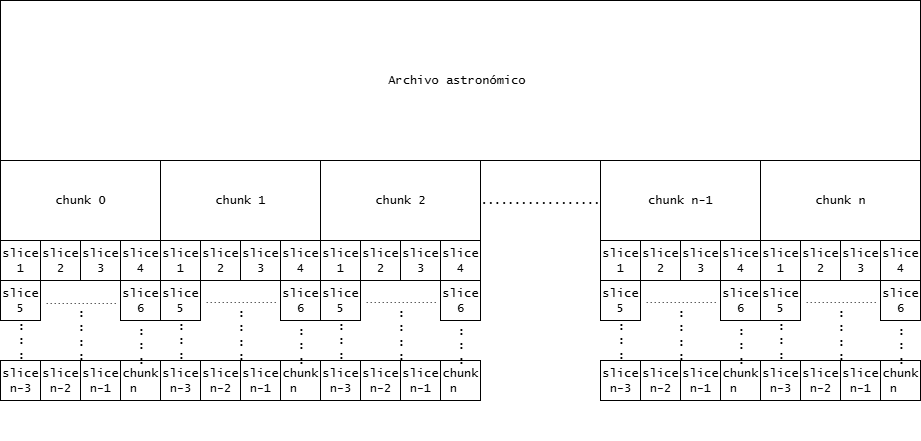
\includegraphics[width=0.9\textwidth]{figures/sistema-chunks.png}
\caption{Esquema de un archivo astronómico dividido en chunks y slices, ilustrando el concepto de procesamiento con solapamiento. Fuente: Elaboración propia.}
\label{fig:sistema-chunks}
\end{figure}

\subsubsection{Aceleración y Control de Recursos}

Vectorización de operaciones matemáticas críticas, integración opcional de procesamiento GPU para algoritmos intensivos en cómputo, y paralelización de bloques de procesamiento para maximizar la utilización de recursos computacionales disponibles. Se implementan \textit{caches} por canal y reducción de I/O para optimizar el rendimiento.

\subsubsection{Registro, Auditoría y Salidas Estandarizadas}

Sistema de \emph{logging} estructurado que registra todas las operaciones críticas, implementación de semillas fijas para algoritmos estocásticos, generación de firmas criptográficas para datos y modelos, y producción de resúmenes de métricas por ejecución para garantizar auditoría completa.

Las salidas incluyen reportes CSV/Parquet estructurados, figuras consistentes (tiempo--DM, dispersado/dedispersado, parches) y \textit{composites} que facilitan el análisis posterior y la validación de resultados.

\begin{table}[H] 
\centering 
  \caption{\label{tab:mejoras} Resumen de mejoras de ingeniería (DRAFTS++). \textit{Fuente: Elaboración propia}.}
\begin{tabular}{p{0.28\textwidth} p{0.32\textwidth} p{0.32\textwidth}} 
\toprule 
    \textbf{Aspecto} & \textbf{Antes (prototipo)} & \textbf{Después (DRAFTS++)} \\
\midrule 
Estructura & Scripts sueltos & Módulos + CLI + configs validadas \\ 
    Archivos grandes & Lectura monolítica & \emph{Chunking} + \emph{overlap} + control de memoria \\
    Detección & Sólo DL (DM--Time) & \emph{Strategy} intercambiable (DM--Time/TWL/SNR) \\
Auditoría & Log mínimo & Log estructurado + semillas + hashes \\ 
    Salidas & Figuras ad hoc & CSV/Parquet + plots estándar + composites \\
\bottomrule 
\end{tabular} 
\end{table}

\subsection{Bloque 2: Extensión a Alta Frecuencia - Cuatro Líneas de Investigación}

Este bloque explora estrategias metodológicas para extender las capacidades de detección hacia regímenes de alta frecuencia (30-100 GHz), donde las firmas dispersivas tradicionales se atenúan significativamente. La detección de FRBs en el régimen milimétrico presenta desafíos fundamentales que requieren aproximaciones metodológicas diferenciadas.

A estas frecuencias, la dispersión temporal se atenúa significativamente debido a la dependencia cuadrática inversa con la frecuencia, resultando en firmas dispersivas que pueden ser indistinguibles del ruido instrumental en resoluciones temporales típicas. Este bloque presenta cuatro líneas de investigación complementarias que abordan diferentes aspectos del desafío de detección en el espectro milimétrico.

\subsubsection{Línea 1: Validación de DRAFTS++ Sin Modificaciones}

\paragraph{Objetivo y Metodología}

Esta línea de investigación busca validar si DRAFTS++ con su arquitectura original (CenterNet en mapas DM-tiempo) puede mantener eficiencia aceptable en regímenes de alta frecuencia. Aunque se anticipa una reducción en el rendimiento debido a la atenuación de las firmas dispersivas, esta validación establece la línea base para comparar las mejoras de las otras líneas.

\paragraph{Criterio Físico para Evaluación}

Se utiliza el retardo dispersivo esperado frente a la resolución temporal como criterio de evaluación:
\[
\Delta t_{\mathrm{ms}} = 4.148808 \times 10^{3}\ \mathrm{DM}\,(\nu_{\mathrm{low}}^{-2}-\nu_{\mathrm{high}}^{-2}) \, .
\]

Cuando $\Delta t_{\mathrm{ms}} < \alpha\, t_{\mathrm{samp}}$ (p.ej., $\alpha\!=\!1.5$), el \textit{bow-tie} no sería resoluble y se espera una degradación significativa del rendimiento.

\subsubsection{Línea 2: Detección por SNR + Clasificación Binaria}

\paragraph{Metodología Híbrida}

Esta línea implementa una aproximación híbrida que combina la detección tradicional por SNR (similar a pipelines clásicos como PRESTO \cite{ransom_presto}) con la red de clasificación binaria de DRAFTS++. El proceso sigue estos pasos:

\begin{enumerate}
\item \textbf{Perfil temporal:} $s(t)$ $\rightarrow$ normalización robusta (mediana/MAD) $\rightarrow$ \textbf{SNR}(t)
\item \textbf{Detección de picos:} Hallazgo de máximos locales $\ge T$ con separación mínima $\Delta t_{\min}$
\item \textbf{Generación de cajas:} Para cada pico $t_i$: generar \textbf{caja sintética} $[t_i-w,\, t_i+w]$
\item \textbf{Dedispersión local:} Construir parche tiempo--frecuencia y dedispersar en rejilla local de DM
\item \textbf{Clasificación binaria:} Usar la red de clasificación de DRAFTS++ para determinar BURST/NO BURST
\item \textbf{Validación DM-aware:} Exigir DM$^\ast\!>\!0$ con incertidumbre acotada
\end{enumerate}

\paragraph{Ventajas de la Aproximación Híbrida}

Esta línea mantiene la eficiencia computacional de la detección por SNR (O(N)) mientras aprovecha la precisión de la red de clasificación entrenada de DRAFTS++. La activación automática del modo HF cuando $\Delta t_{\mathrm{ms}} < \alpha\, t_{\mathrm{samp}}$ garantiza que se use la estrategia más apropiada según las condiciones físicas.

\begin{figure}[H] 
\centering 
% \includegraphics[width=0.9\textwidth]{hf_mode_snr_boxes.pdf} 
\caption{\label{fig:hf} Modo HF: del perfil SNR a cajas sintéticas, dedispersión local y clasificación binaria. Fuente: Elaboración propia.} 
\end{figure}

\paragraph{Pseudocódigo de Detección SNR}

\begin{algorithm}[H]
\caption{Detección SNR para Alta Frecuencia}
\begin{algorithmic}[1]
\Input{$s(t)$, umbral $T$, separación mínima $\Delta t_{min}$}
\Output{Lista de picos candidatos $\{t_i\}$}
\Function{DetectarPicosSNR}{$s$, $T$, $\Delta t_{min}$}
    \State $s_{norm} \leftarrow (s - median(s)) / MAD(s)$
    \State $picos \leftarrow maxima\_locales(s_{norm})$
    \State $candidatos \leftarrow [\ ]$
    \For{$t$ \textbf{in} $picos$}
        \If{$s_{norm}[t] \geq T$ \textbf{and} $dist\_minima(t, candidatos) \geq \Delta t_{min}$}
            \State $candidatos.append(t)$
        \EndIf
    \EndFor
    \State \textbf{return} $candidatos$
\EndFunction
\end{algorithmic}
\end{algorithm}

\subsubsection{Línea 3: Nuevos Plots Característicos - TWL-maps}

\paragraph{Concepto de TWL-maps}

En el régimen de alta frecuencia, donde las firmas dispersivas tradicionales se atenúan significativamente, los mapas tiempo--ancho--polarización lineal (TWL) proporcionan información diagnóstica complementaria que puede compensar la pérdida de evidencia dispersiva. Estos productos especializados aprovechan la información de polarización disponible en observaciones con datos de Stokes completos.

\paragraph{Análisis de Polarización Lineal}

Cuando se dispone de datos de Stokes $I,Q,U$ \cite{hamaker1996understanding}, se puede calcular la \textbf{polarización lineal} $L=\sqrt{Q^2+U^2}$, que cuantifica la intensidad de la componente polarizada de la señal electromagnética. Esta medida proporciona información adicional sobre la naturaleza física de las fuentes y puede revelar patrones que no son evidentes en el análisis de intensidad total únicamente.

\paragraph{Flujo de Detección Híbrida TWL}

El proceso de detección híbrida sigue una secuencia específica que garantiza robustez y eficiencia:

\begin{enumerate}
\item \textbf{Evaluación de disponibilidad TWL:} El sistema verifica si \texttt{TWL\_HYBRID\_DETECTION} está habilitado y si los datos de polarización (Stokes Q, U) están disponibles.
\item \textbf{Generación de mapa t-W:} Si la detección híbrida está activa, se genera el mapa tiempo-ancho de ocupación de banda mediante \texttt{generate\_twl\_map\_for\_window}.
\item \textbf{Conversión a tensor RGB:} El mapa 2D se convierte a un tensor RGB de 512×512 píxeles usando \texttt{twl\_occupancy\_to\_detection\_tensor} para compatibilidad con CenterNet.
\item \textbf{Detección con CenterNet:} El tensor se procesa con la red de detección para identificar candidatos potenciales.
\item \textbf{Evaluación de candidatos:} Si se encuentran candidatos, se procede a clasificación binaria; si no, se activa el fallback SNR.
\item \textbf{Fallback SNR:} En caso de fallo de la detección híbrida o si está deshabilitada, se ejecuta \texttt{compute\_snr\_profile} y \texttt{\_find\_snr\_peaks} para detección tradicional.
\item \textbf{Clasificación final:} Todos los candidatos (híbridos o SNR) pasan por \texttt{classify\_patch} para determinar si son BURST o NO BURST.
\item \textbf{Guardado de resultados:} Los candidatos válidos se almacenan con métricas completas y se generan visualizaciones correspondientes.
\end{enumerate}

\begin{figure}[H]
\centering
\begin{tikzpicture}[
    node distance=1.2cm and 1.5cm,
    box/.style={rectangle, draw, fill=blue!20, text width=2.2cm, text centered, minimum height=0.7cm, font=\small},
    decision/.style={diamond, draw, fill=yellow!20, text width=1.8cm, text centered, minimum height=0.7cm, font=\small},
    process/.style={rectangle, draw, fill=green!20, text width=2.2cm, text centered, minimum height=0.7cm, font=\small},
    arrow/.style={-Stealth, thick}
]

% Nodos principales
\node[box] (A) {Pipeline Alta Frecuencia};
\node[decision, below=of A] (B) {TWL Híbrido?};
\node[process, below left=of B] (C) {Generar Mapa t-W};
\node[process, below=of C] (D) {Convertir a Tensor RGB};
\node[process, below=of D] (E) {Red de Detección};
\node[decision, below=of E] (F) {Candidatos?};
\node[process, below left=of F] (G) {Clasificación Binaria};
\node[process, below right=of B] (H) {Fallback SNR};
\node[process, below=of H] (I) {Detección SNR Tradicional};
\node[process, below=of G] (J) {Guardar Candidatos};

% Conexiones
\draw[arrow] (A) -- (B);
\draw[arrow] (B) -- node[left] {Sí} (C);
\draw[arrow] (C) -- (D);
\draw[arrow] (D) -- (E);
\draw[arrow] (E) -- (F);
\draw[arrow] (F) -- node[left] {Sí} (G);
\draw[arrow] (B) -- node[right] {No} (H);
\draw[arrow] (H) -- (I);
\draw[arrow] (I) -- (F);
\draw[arrow] (G) -- (J);

\end{tikzpicture}
\caption{\label{fig:hf-pipeline} Flujo del Pipeline de Alta Frecuencia: detección híbrida TWL con fallback automático a SNR tradicional. El diagrama muestra la decisión que determina si usar detección híbrida (mapa t-W + CenterNet) o fallback a SNR tradicional. Fuente: Elaboración propia.}
\end{figure}

\begin{figure}[H] 
\centering 
% \includegraphics[width=0.9\textwidth]{twl_map.pdf} 
\caption{\label{fig:twl} Ejemplo de TWL-map (tiempo vs. ancho con intensidad de $L$). Fuente: Elaboración propia.} 
\end{figure}

\subsubsection{Línea 4: Estrategias Alternativas del Autor de DRAFTS}

\paragraph{DM-range Expand \& Step Coarse}

Esta línea explora estrategias sugeridas por Yong–Kun Zhang \cite{zhang2024drafts} para maximizar la visibilidad de firmas dispersivas residuales. La metodología incluye:

\begin{itemize}
\item \textbf{Expansión del rango/step de DM:} Ampliar el rango y el \textit{step} de DM hasta "abrir" el \textit{bow-tie}
\item \textbf{Verificación estadística:} Una vez detectado, exigir centro con DM$>0$ significativamente mayor que cero
\item \textbf{Detección de candidatos cerca de DM$\approx 0$:} Mediante algoritmos de detección de picos adaptativos seguida de validación rigurosa
\end{itemize}

\paragraph{Fishing en DM$\approx 0$ + Chequeos Estrictos}

\textit{Pescar} candidatos con clasificador o detector simple cerca de DM$\approx 0$; luego validar con DM$>0$, consistencia por sub-bandas y coherencia entre \emph{chunks}. Útil para eventos débiles sin \textit{bow-tie} claro.

\paragraph{Integración con el Pipeline}

Ambas tácticas se exponen como \textbf{estrategias} de propuesta de candidatos (alternativas a SNR/TWL/DM--Time) y se someten al \textbf{mismo} validador DM-aware, clasificación y visualización.

\begin{table}[H] 
\centering 
\caption{\label{tab:estrategias} Estrategias de propuesta de candidatos y criterios de uso. Fuente: Elaboración propia.} 
\begin{tabular}{p{0.24\textwidth} p{0.38\textwidth} p{0.30\textwidth}} 
\toprule 
\textbf{Estrategia} & \textbf{Cuándo usarla} & \textbf{Pros / Contras} \\ 
\midrule 
CenterNet en DM--Time & $\Delta t \gg t_{\rm samp}$ (bow-tie resoluble) & + Precisa en L/S-band; -- Pierde poder en mm-wave \\ 
TWL-Híbrido + CenterNet & Stokes disponibles en mm-wave & + Usa polarización/anchos; -- Coste extra de features \\ 
SNR-only + Clasificador & mm-wave sin bow-tie claro & + O(N), simple; -- Más FP sin validación DM-aware \\ 
DM$\approx 0$ fishing + validar DM$>0$ & Para "pescar" candidatos débiles & + Sensible; -- Requiere validaciones estrictas \\ 
\bottomrule 
\end{tabular} 
\end{table}

\begin{table}[H]
  \centering
  \caption{\label{tab:param_hf} Parámetros del modo HF (valores iniciales). \textit{Fuente: Elaboración propia}.}
  \begin{tabular}{p{0.35\textwidth} p{0.55\textwidth}}
    \toprule
    \textbf{Parámetro} & \textbf{Descripción} \\
    \midrule
    $T$ (umbral SNR) & 5--7; ajustar por FDR y condiciones de ruido \\
    $\Delta t_{\min}$ & Múltiplo del ancho de pulso esperado \\
    Rejilla DM local & Centrada en 0; pasos gruesos y posterior refinamiento \\
    Sub-bandas & 2--4 particiones para coherencia \\
    Criterio DM & Requerir DM$^\ast>0$ (con error acotado) \\
    \bottomrule
  \end{tabular}
\end{table}

\subsection{Arquitectura Unificada y Diagramas}

\subsubsection{Arquitectura Unificada (Strategy + Validator + Visualizer)}

Se adopta un patrón \textbf{Strategy} para la \textbf{propuesta de candidatos} (intercambiable: DM--Time/CenterNet, TWL-híbrido, SNR, DM-expand, fishing en DM$\approx0$), con un \textbf{validador DM-aware} común y un \textbf{visualizador desacoplado}. La función de proceso se unifica como \texttt{process\_slice(..., strategy)}.

\begin{figure}[H] 
\centering 
% \includegraphics[width=0.96\textwidth]{arquitectura_unificada.pdf} 
\caption{\label{fig:arquitectura-unificada} Arquitectura unificada: Strategy (propuesta de candidatos) + Validador DM-aware + Visualizador. \textit{Fuente: Elaboración propia}.} 
\end{figure}

\paragraph{Bucle Unificado (Pseudocódigo)}

\begin{algorithm}[H]
\caption{Pipeline Unificado con Strategy Pattern}
\begin{algorithmic}[1]
\Input{$config$, $obs\_params$, $data\_files$}
\Output{Candidatos validados y métricas}
\Function{RunPipeline}{$config$, $obs\_params$}
    \State $strategy \leftarrow select\_strategy(config, obs\_params)$
    \For{$chunk$ \textbf{in} $stream\_data(\ldots)$}
        \State $cands \leftarrow strategy.propose(chunk, meta)$
        \For{$c$ \textbf{in} $cands$}
            \State $patch \leftarrow extract\_patch\_and\_dedisperse(chunk, c, local\_dm\_grid)$
            \State $y \leftarrow classifier.predict(patch)$
            \If{$y.is\_burst$ \textbf{and} $dm\_validate(patch)$ \textbf{and} $subband\_consistency(patch)$}
                \State $save\_candidate(patch, y, metrics)$
            \EndIf
        \EndFor
    \EndFor
    \State $visualize\_and\_summarize(run\_id)$
\EndFunction
\end{algorithmic}
\end{algorithm}

\subsubsection{Diagrama End-to-End del Pipeline}

La Figura \ref{fig:pipeline-end-to-end} sintetiza el flujo desde \texttt{main.py} hasta los resultados, con ramas clásica (DM--Time/CenterNet) y de alta frecuencia (TWL-híbrido, SNR) y \textit{fallbacks}.

\begin{figure}[H]
\centering
\begin{tikzpicture}[
    node distance=1.0cm and 1.5cm,
    box/.style={rectangle, draw, fill=blue!20, text width=2.0cm, text centered, minimum height=0.6cm, font=\tiny},
    decision/.style={diamond, draw, fill=yellow!20, text width=1.6cm, text centered, minimum height=0.6cm, font=\tiny},
    process/.style={rectangle, draw, fill=green!20, text width=2.0cm, text centered, minimum height=0.6cm, font=\tiny},
    output/.style={rectangle, draw, fill=orange!20, text width=2.0cm, text centered, minimum height=0.6cm, font=\tiny},
    arrow/.style={-Stealth, thick}
]

% FLUJO SIMPLIFICADO
\node[box] (A) {main.py};
\node[box, below=of A] (B) {run\_pipeline};
\node[box, below=of B] (C) {Cargar Modelos};

% ENTRADA DE DATOS
\node[box, right=of B] (D) {find\_data\_files};
\node[decision, below=of D] (E) {Tipo Archivo?};
\node[box, below left=of E] (F) {fits\_handler};
\node[box, below right=of E] (G) {filterbank\_handler};

% PROCESAMIENTO
\node[box, below=of E] (H) {streaming\_orchestrator};
\node[box, below=of H] (I) {Procesar Chunk};
\node[decision, below=of I] (J) {Frecuencia ≥ 8GHz?};

% PIPELINES
\node[box, below left=of J] (K) {Pipeline Alta Frecuencia};
\node[box, below right=of J] (L) {Pipeline Clásico};

% DETECCIÓN
\node[decision, below=of K] (M) {TWL\_HYBRID?};
\node[box, below left=of M] (N) {TWL + CenterNet};
\node[box, below right=of M] (O) {SNR Tradicional};
\node[process, below=of L] (P) {CenterNet DM-Time};

% CLASIFICACIÓN
\node[process, below=of N] (Q) {classify\_patch};
\node[process, below=of O] (R) {classify\_patch};
\node[process, below=of P] (S) {classify\_patch};

% RESULTADOS
\node[output, below=of Q] (T) {Guardar Candidatos};
\node[output, below=of R] (U) {Guardar Candidatos};
\node[output, below=of S] (V) {Guardar Candidatos};

% VISUALIZACIÓN
\node[output, below=of T] (W) {Plots + CSV};
\node[output, below=of U] (X) {Plots + CSV};
\node[output, below=of V] (Y) {Plots + CSV};

% Conexiones principales
\draw[arrow] (A) -- (B);
\draw[arrow] (B) -- (C);
\draw[arrow] (B) -- (D);
\draw[arrow] (D) -- (E);
\draw[arrow] (E) -- node[left] {FITS} (F);
\draw[arrow] (E) -- node[right] {Filterbank} (G);
\draw[arrow] (F) -- (H);
\draw[arrow] (G) -- (H);
\draw[arrow] (H) -- (I);
\draw[arrow] (I) -- (J);
\draw[arrow] (J) -- node[left] {Sí} (K);
\draw[arrow] (J) -- node[right] {No} (L);

% Detección
\draw[arrow] (K) -- (M);
\draw[arrow] (M) -- node[left] {Sí} (N);
\draw[arrow] (M) -- node[right] {No} (O);
\draw[arrow] (L) -- (P);

% Clasificación
\draw[arrow] (N) -- (Q);
\draw[arrow] (O) -- (R);
\draw[arrow] (P) -- (S);

% Resultados
\draw[arrow] (Q) -- (T);
\draw[arrow] (R) -- (U);
\draw[arrow] (S) -- (V);

% Visualización
\draw[arrow] (T) -- (W);
\draw[arrow] (U) -- (X);
\draw[arrow] (V) -- (Y);

\end{tikzpicture}
\caption{\label{fig:pipeline-end-to-end} Diagrama end-to-end (ingesta $\to$ \emph{streaming}/\emph{chunking} $\to$ estrategia de candidatos $\to$ clasificación/validación $\to$ visualización y salida). \textit{Fuente: Elaboración propia}.}
\end{figure}

\subsection{Evaluación y Métricas}

Conjuntos ya analizados (control de \emph{recall}) y datos mm-wave piloto. Métricas: \emph{recall}, \emph{precision}, tasa de FP, latencia por GB, throughput, coherencia sub-bandas y \emph{chunks}. \emph{Ablation}: sin validación DM-aware, sin coherencia por sub-bandas, sin TWL.

\subsection{Síntesis de Contribuciones}

\subsubsection{Resumen de los Dos Bloques Principales}

Esta propuesta establece una transformación fundamental en la metodología de detección de FRBs, evolucionando desde un prototipo de investigación hacia un sistema productivo de clase observacional. Las contribuciones presentadas abordan tanto aspectos de ingeniería de software como innovaciones metodológicas específicas para el régimen milimétrico.

\textbf{Bloque 1: DRAFTS++} establece los fundamentos arquitectónicos para operaciones productivas mediante una refactorización sistemática que implementa modularización especializada, procesamiento eficiente por chunks, trazabilidad completa y artefactos de salida estandarizados. Esta transformación garantiza escalabilidad computacional, reproducibilidad experimental y mantenibilidad del sistema en entornos observacionales reales.

\textbf{Bloque 2: Extensión a Alta Frecuencia} extiende las capacidades de detección hacia regímenes de alta frecuencia mediante la implementación de cuatro líneas de investigación complementarias que abordan diferentes aspectos del desafío de detección en el espectro milimétrico. Esta extensión metodológica compensa las limitaciones físicas inherentes a la detección dispersiva en el espectro milimétrico y establece nuevas vías de investigación basadas en propiedades de polarización.

\subsubsection{Perspectivas Futuras}

Esta investigación establece las bases para la próxima generación de sistemas de detección de FRBs, combinando robustez operacional con innovación metodológica. Los desarrollos futuros incluirán:

\begin{itemize}
\item \textbf{Reentrenamiento de modelos:} Una vez identificados nuevos plots característicos efectivos (como TWL-maps), se procederá al reentrenamiento de las redes neuronales o creación de nuevos modelos específicamente optimizados para estos productos diagnósticos.
\item \textbf{Integración de técnicas de aprendizaje automático avanzadas:} Incorporación de arquitecturas más sofisticadas y técnicas de data augmentation específicas para el dominio astronómico.
\item \textbf{Extensión a otros regímenes espectrales:} Aplicación de las metodologías desarrolladas a otros rangos de frecuencia y tipos de transientes.
\item \textbf{Aplicación a programas observacionales de gran escala:} Implementación en observatorios reales para validación operacional completa.
\end{itemize}

Las figuras \ref{fig:pipeline-end-to-end}, \ref{fig:hf-pipeline}, \ref{fig:hf}, \ref{fig:twl} y \ref{fig:arquitectura-unificada} documentan la evolución arquitectónica completa, desde la conceptualización inicial hasta la implementación productiva. Juntas, demuestran no solo la transformación técnica del sistema, sino la creación de una plataforma extensible que puede adaptarse a futuros desarrollos en radioastronomía de transientes (Fuente: Elaboración propia).
\newpage
\secnumbersection{VALIDACIÓN DE LA SOLUCIÓN}

La validación de la solución propuesta constituye una etapa crítica que permite demostrar la efectividad de los dos bloques desarrollados en diferentes entornos y condiciones. Esta validación se estructura en dos componentes principales: la validación del bloque de bajas frecuencias (DRAFTS++) y la validación del bloque de altas frecuencias (High Frequency Detection).

\subsection{VALIDACIÓN DEL BLOQUE DE BAJAS FRECUENCIAS (DRAFTS++)}

La validación de DRAFTS++ se realizó mediante un proceso incremental que permitió verificar cada componente del sistema antes de su implementación completa. Este enfoque metodológico aseguró la robustez y confiabilidad del pipeline desarrollado.

\subsubsection{Validación Inicial con Dataset de Entrenamiento}

El proceso de validación inició con el dataset FAST-FREX (FAST dataset for Fast Radio bursts EXploration), el mismo conjunto de datos utilizado para el entrenamiento de los modelos de detección. Esta etapa fue fundamental para validar todas las nuevas funcionalidades implementadas en DRAFTS++, incluyendo los nuevos tipos de visualización y el manejo de archivos de entrada, antes incluso del desarrollo del sistema de chunking.

\begin{figure}[H]
    \centering
    \includegraphics[width=\textwidth]{figures/FRB20180301_0001_slice003.png}
    \caption{Detección de un Fast Radio Burst (FRB) del dataset de entrenamiento FAST-FREX. El panel superior muestra el mapa de dispersión (DM vs. Tiempo) con el evento resaltado. Los paneles inferiores presentan el SNR en cascada crudo, el SNR dedispersado y el SNR del parche candidato, confirmando una detección robusta con un SNR de 5.9$\sigma$.}
    \label{fig:frb20180301_0001_slice003}
\end{figure}

\begin{figure}[H]
    \centering
    \includegraphics[width=\textwidth]{figures/FRB20201124_0009_slice004.png}
    \caption{Detección de un segundo Fast Radio Burst (FRB) del dataset de entrenamiento FAST-FREX. Se observa una detección robusta con SNR de 16.5$\sigma$ después de la dedispersión, confirmando la efectividad del sistema en el dataset de entrenamiento.}
    \label{fig:frb20201124_0009_slice004}
\end{figure}

\subsubsection{Validación de Continuidad Temporal y Time Domain}

Una vez establecida la funcionalidad básica, se procedió a evaluar una característica crítica para cualquier pipeline de detección: la continuidad temporal y la precisión en el dominio del tiempo. Para esta validación se utilizó el pulsar de prueba B0355+54\_FB\_20220918, seleccionado por sus características ideales para este propósito:

\begin{itemize}
    \item \textbf{Brightness}: Pulsar sumamente brillante que facilita la detección
    \item \textbf{Periodo de rotación}: 0.156 segundos
    \item \textbf{Duración del archivo}: 117.23 segundos (1 minuto 57 segundos)
    \item \textbf{Pulsos esperados}: 752 pulsos teóricos
\end{itemize}

Los resultados obtenidos fueron altamente satisfactorios:
\begin{itemize}
    \item \textbf{Pulsos detectados}: 732 de 752 esperados (97.3\% de eficiencia)
    \item \textbf{Clasificación}: 718 clasificados como BURSTS, 14 como NO BURSTS
\end{itemize}

\begin{figure}[H]
    \centering
    \includegraphics[width=\textwidth]{figures/B0355+54_FB_20220918_slice000.png}
    \caption{Validación de continuidad temporal - Slice 000: Se observan 7 pulsos detectados en el primer segundo de observación, demostrando la capacidad del sistema para detectar eventos periódicos con alta precisión temporal. Todos los pulsos fueron clasificados como BURSTS con scores de clasificación superiores a 0.99.}
    \label{fig:b0355_slice000}
\end{figure}


\begin{figure}[H]
    \centering
    \includegraphics[width=\textwidth]{figures/B0355+54_FB_20220918_slice001.png}
    \caption{Validación de continuidad temporal - Slice 001: Continuidad perfecta en el segundo slice, mostrando 5 pulsos clasificados como BURSTS y 1 como NO BURST. La consistencia en la detección temporal confirma la robustez del sistema de procesamiento por ventanas.}
    \label{fig:b0355_slice001}
\end{figure}

Este resultado confirmó la capacidad del sistema para mantener la continuidad temporal entre ventanas de procesamiento y validó la precisión de las redes de detección pre-entrenadas de DRAFTS en condiciones controladas.

\begin{figure}[H]
    \centering
    \includegraphics[width=\textwidth]{figures/B0355+54_FB_20220918_slice013.png}
    \caption{Caso de estudio: Pulso dudoso en la clasificación. El evento \#6 (DM: 55.5, Time: 13.93s) muestra un score de detección alto (0.73) pero un score de clasificación bajo (0.27), resultando en clasificación "NO BURST". El evento \#4 (DM: 54.6, Time: 14.08s) presenta un score de detección muy alto (0.81) pero clasificación muy baja (0.09). Esto demuestra la capacidad del sistema para detectar señales ambiguas que requieren revisión manual.}
    \label{fig:b0355_slice013}
\end{figure}

\subsubsection{Validación con Datos del FRB 121102}

Para evaluar el rendimiento del sistema en condiciones reales y con archivos de gran tamaño, se utilizó el dataset del FRB 121102, basado en el trabajo de \cite{cruces2020frb121102}. Este dataset presentó desafíos computacionales significativos que requirieron la implementación del sistema de chunking y la optimización del consumo de recursos.

\paragraph{Metodología de Validación}

La validación se realizó mediante una comparación directa con los resultados reportados en la literatura por Cruces et al. (2020) \cite{cruces2020frb121102}, quienes estudiaron el comportamiento repetitivo de FRB 121102 incluyendo periodicidad, tiempos de espera y distribución de energía. Se analizaron los mismos archivos de observación para asegurar una evaluación equitativa.

\paragraph{Resultados de Detección del Pipeline DRAFTS++}

El análisis de FRB121102 con el pipeline DRAFTS++ produjo 41 detecciones distribuidas en 6 archivos de observación (3096, 3098, 3099, 3100, 3101, 3102). Los resultados se clasificaron en tres categorías principales:

\begin{enumerate}
    \item \textbf{Bursts confirmados por literatura} (24 eventos): Detectados tanto por DRAFTS++ como reportados por Cruces et al. (2020)
    \item \textbf{Nuevos candidatos sin confirmar} (15 eventos): Detectados únicamente por DRAFTS++, pendientes de validación científica
    \item \textbf{Nuevos eventos confirmados} (2 eventos): Detectados por DRAFTS++ y 100\% confirmados por el grupo de astrónomos colaboradores
\end{enumerate}

\subparagraph{Bursts Confirmados por Literatura}

Los 24 bursts que fueron detectados tanto por el pipeline DRAFTS++ como reportados en la literatura por Cruces et al. (2020) se presentan en detalle en el Anexo A (Tabla \ref{tab:anexo_confirmed_bursts}), demostrando la capacidad del sistema para identificar correctamente eventos conocidos.

\subparagraph{Nuevos Candidatos Sin Confirmar}

Los 15 nuevos candidatos detectados únicamente por DRAFTS++ que aún requieren confirmación científica se presentan en detalle en el Anexo A (Tabla \ref{tab:anexo_candidate_bursts}). Estos representan el potencial de descubrimiento del sistema.

\subparagraph{Nuevos Eventos Confirmados}

Los 2 nuevos eventos de bursts que fueron detectados por DRAFTS++ y posteriormente 100\% confirmados por el grupo de astrónomos colaboradores se presentan en detalle en el Anexo A (Tabla \ref{tab:anexo_new_confirmed_bursts}).

Estos dos nuevos eventos representan descubrimientos científicos genuinos realizados por DRAFTS++, como se muestra en las Figuras \ref{fig:new_event_3096} y \ref{fig:new_event_3102}. Las visualizaciones confirman la detección robusta de ambos eventos con altos valores de SNR después de la dedispersión.

\begin{figure}[H]
    \centering
    \includegraphics[width=\textwidth]{figures/3096_0001_00_8bit_slice039.png}
    \caption{Primer nuevo evento confirmado de FRB121102 detectado por DRAFTS++ en el archivo 3096\_0001\_00\_8bit, slice 039. El evento muestra DM=563.6 pc cm$^{-3}$ y Time=2421.559296s, con un SNR de 6.3$\sigma$ después de la dedispersión. La detección fue 100\% confirmada por el grupo de astrónomos colaboradores. \textit{Fuente: Elaboración propia}.}
    \label{fig:new_event_3096}
\end{figure}

\begin{figure}[H]
    \centering
    \includegraphics[width=\textwidth]{figures/3102_0001_00_8bit_slice040.png}
    \caption{Segundo nuevo evento confirmado de FRB121102 detectado por DRAFTS++ en el archivo 3102\_0001\_00\_8bit, slice 040. El evento muestra DM=564.88 pc cm$^{-3}$ y Time=723.455399s, con un SNR de 12.0$\sigma$ después de la dedispersión. Este evento representa uno de los bursts más brillantes detectados en el dataset y fue 100\% confirmado por el grupo de astrónomos colaboradores. \textit{Fuente: Elaboración propia}.}
    \label{fig:new_event_3102}
\end{figure}

\paragraph{Análisis de Distribución Temporal}

Para visualizar la distribución temporal de los diferentes tipos de detecciones, se generó un histograma que muestra la frecuencia de bursts por archivo de observación. Esta visualización permite identificar patrones en la detección y validar la consistencia del sistema a lo largo de las diferentes sesiones de observación.

\begin{figure}[H]
    \centering
    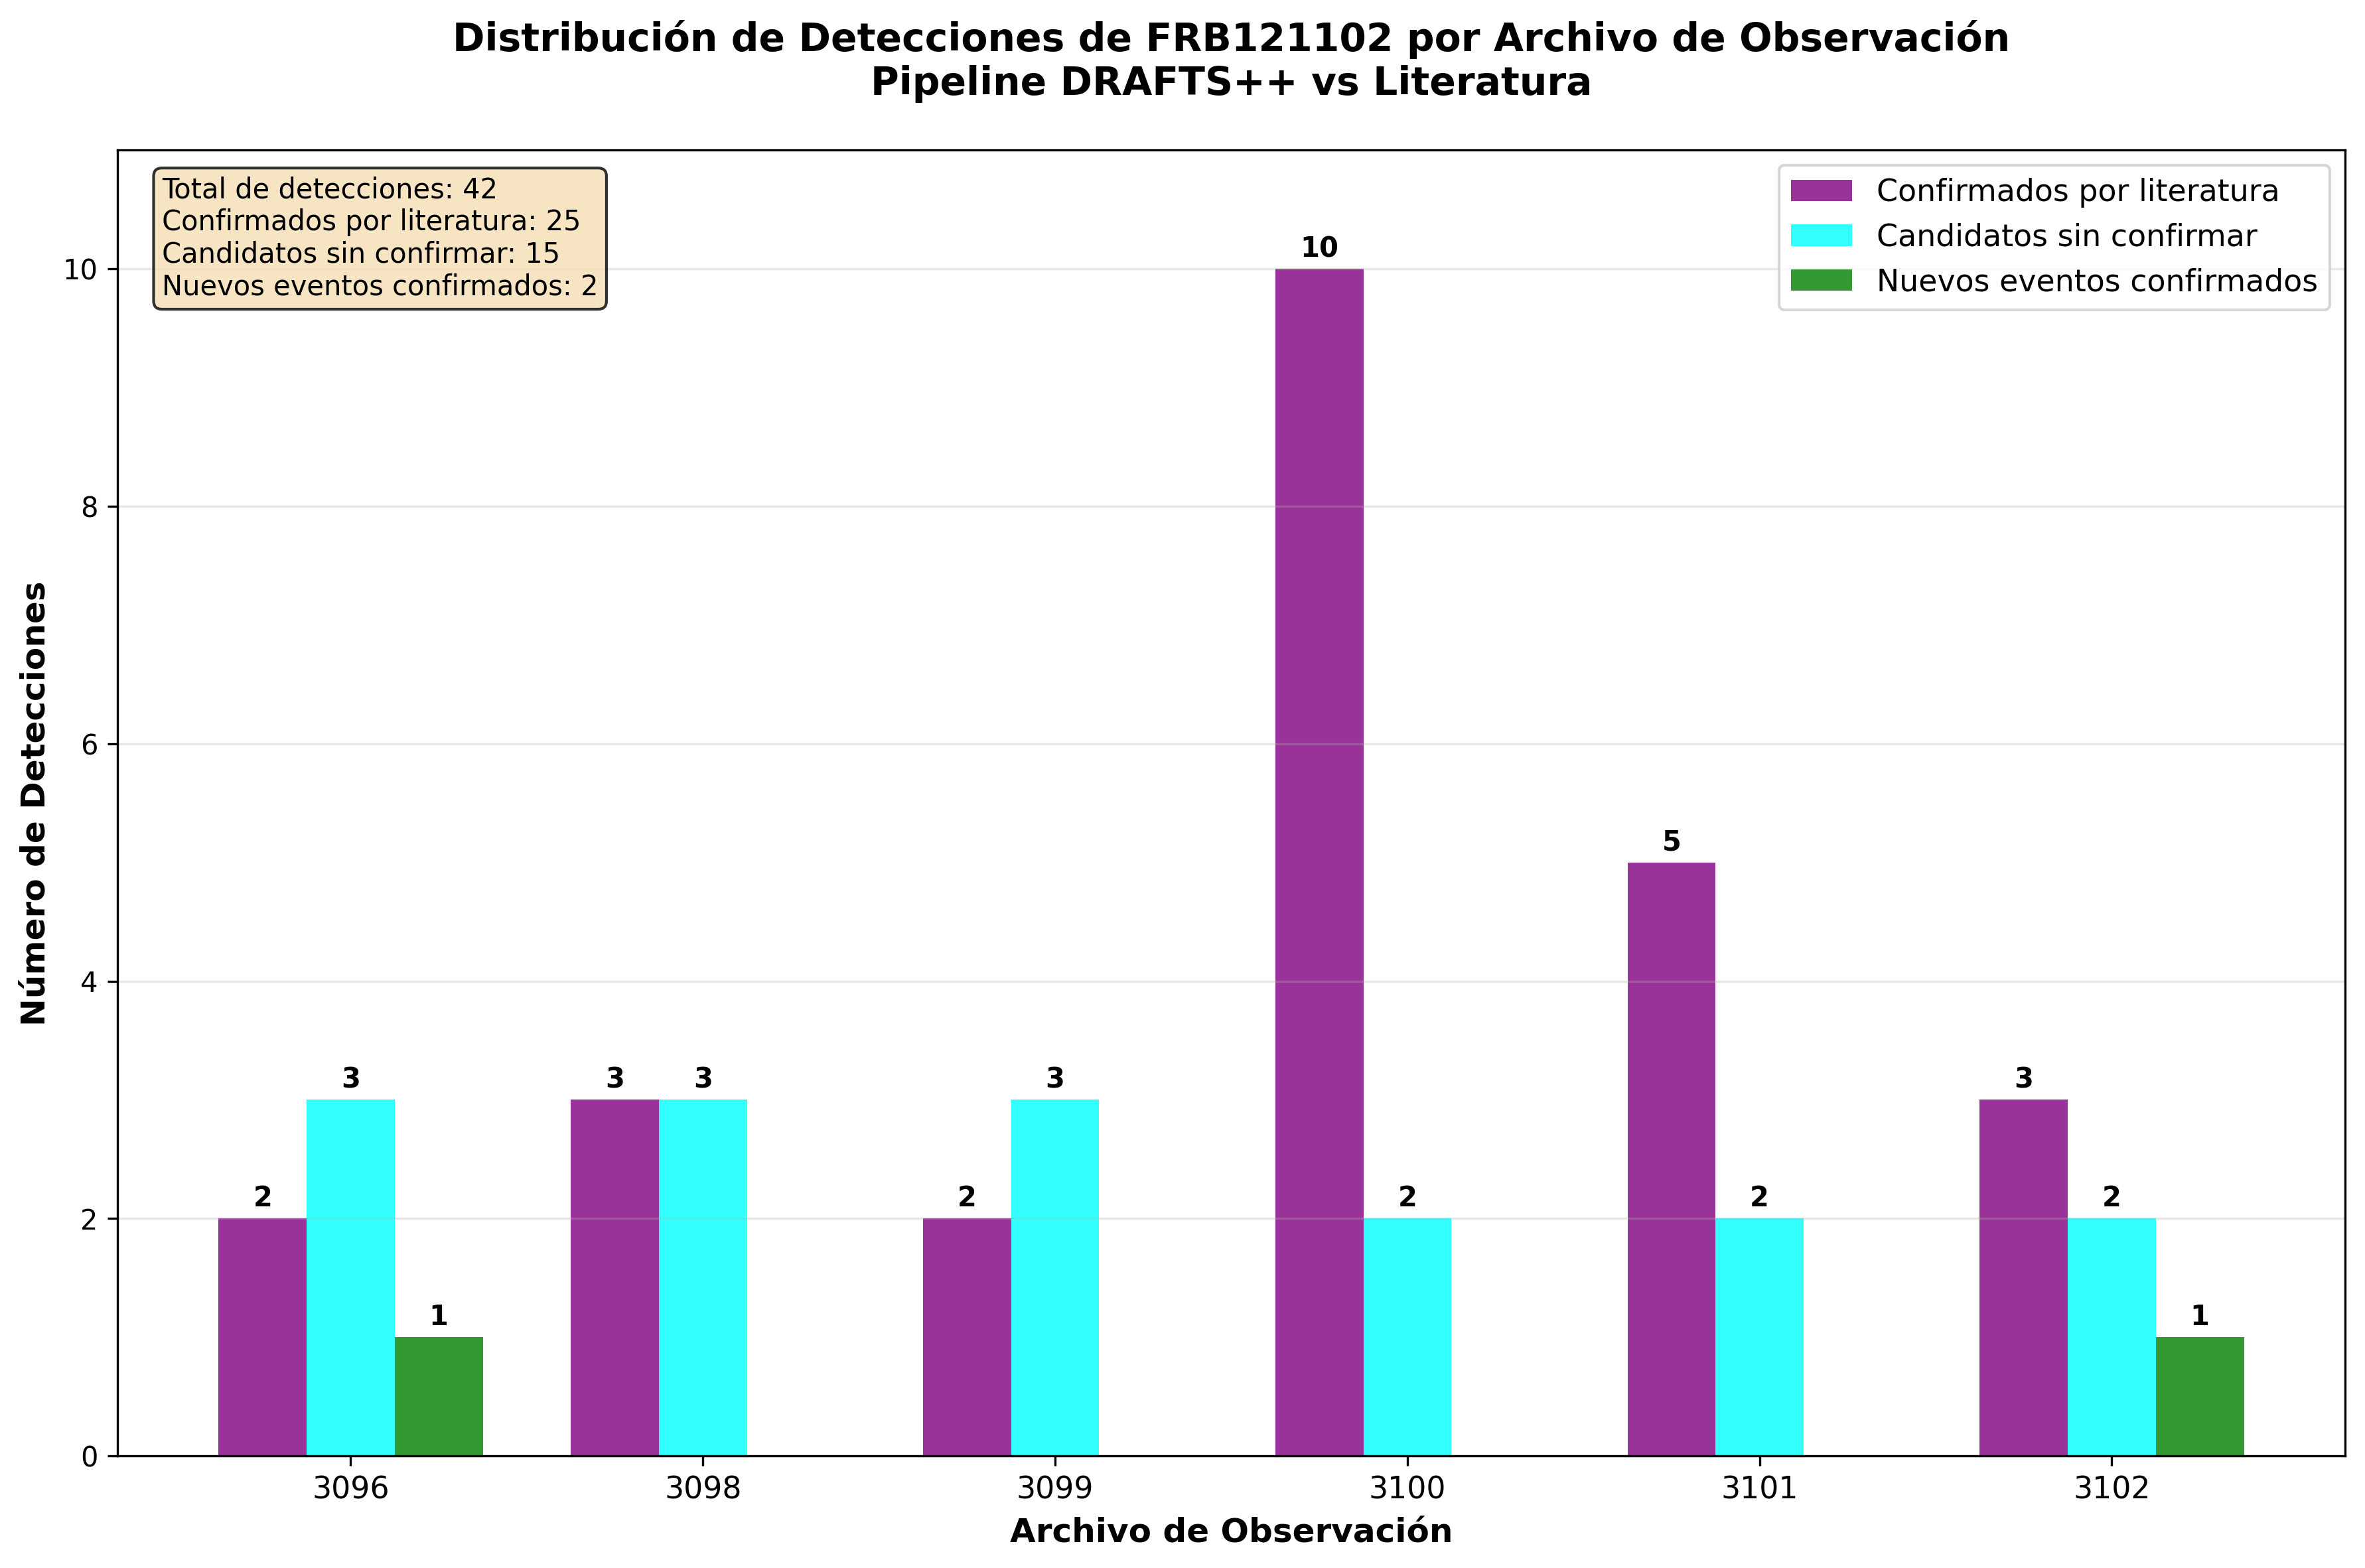
\includegraphics[width=0.8\textwidth]{figures/frb121102_detection_histogram.png}
    \caption{Histograma de distribución de detecciones de FRB121102 por archivo de observación. Las barras muestran: \textcolor{purple}{\textbf{Morado}} = bursts confirmados por literatura, \textcolor{cyan}{\textbf{Celeste}} = nuevos candidatos sin confirmar, \textcolor{green}{\textbf{Verde}} = nuevos eventos confirmados. \textit{Fuente: Elaboración propia}.}
    \label{fig:frb121102_histogram}
\end{figure}

\paragraph{Análisis de Resultados}

Los resultados obtenidos superaron significativamente las expectativas establecidas en la literatura:

\begin{itemize}
    \item \textbf{Bursts de literatura detectados}: 24/24 (100\% de detección) - todos los bursts reportados por Cruces et al. (2020) fueron identificados correctamente por DRAFTS++
    \item \textbf{Nuevos eventos confirmados}: 2 eventos adicionales detectados por DRAFTS++ y 100\% confirmados por el grupo de astrónomos colaboradores
    \item \textbf{Candidatos adicionales}: 15 candidatos nuevos detectados únicamente por DRAFTS++, pendientes de confirmación científica
    \item \textbf{Total de detecciones}: 41 eventos distribuidos en 6 archivos de observación
\end{itemize}

\paragraph{Validación de Funcionalidades}

Esta validación confirmó exitosamente todas las mejoras implementadas en DRAFTS++:

\begin{itemize}
    \item \textbf{Manejo robusto de archivos}: Procesamiento eficiente de archivos FITS y Filterbank de gran tamaño
    \item \textbf{Control de parámetros}: Configuración total por parte del usuario a través del sistema centralizado
    \item \textbf{Continuidad temporal}: Precisión quirúrgica en el manejo de timestamps entre chunks y slices
    \item \textbf{Precisión de detección}: Identificación correcta de todos los eventos conocidos de la literatura
    \item \textbf{Eficiencia computacional}: Sistema de chunking y overlap optimizado para archivos masivos
    \item \textbf{Capacidad de descubrimiento}: Detección de eventos nuevos no reportados previamente
    \item \textbf{Generación de outputs}: Visualizaciones y reportes apropiados para análisis científico
\end{itemize}

\paragraph{Implicaciones Científicas}

Los resultados obtenidos no solo validan la funcionalidad técnica del pipeline DRAFTS++, sino que también contribuyen significativamente al conocimiento científico del campo. La detección de 2 nuevos bursts confirmados y 15 candidatos adicionales representa un avance importante en el estudio de FRB 121102, demostrando la capacidad del sistema para realizar descubrimientos científicos genuinos.

\subsection{VALIDACIÓN DEL BLOQUE DE ALTAS FRECUENCIAS}

La validación del bloque de altas frecuencias se centró en el dataset del observatorio ALMA, específicamente los datos del magnetar del Centro Galáctico PSR J1745-2900, basado en el trabajo de \cite{veracasanova2025}.

\paragraph{Referencia de Validación}

Para esta validación se utilizó como referencia los resultados oficiales reportados por Vera-Casanova et al. (2025), quienes detectaron 8 pulsos del magnetar PSR J1745-2900 en los siguientes archivos y tiempos:

\begin{table}[H]
    \centering
    \caption{Pulsos del magnetar PSR J1745-2900 reportados por Vera-Casanova et al. (2025). \textit{Fuente: Vera-Casanova et al. (2025) \cite{veracasanova2025}.}}
    \label{tab:veracasanova_reference}
    \begin{tabular}{|c|c|}
        \hline
        \textbf{File} & \textbf{Time(s)} \\
        \hline
        142\_0003 & 39.977 \\
        142\_0006 & 10.882 \\
        142\_0006 & 25.829 \\
        153\_0006 & 23.444 \\
        230\_0002 & 2.3 \\
        230\_0002 & 17.395 \\
        230\_0003 & 36.548 \\
        242\_0005 & 44.919 \\
        \hline
    \end{tabular}
\end{table}

\subsubsection{Validación con Pipeline Clásico Adaptado}

La primera línea de validación consistió en aplicar DRAFTS++ y el pipeline clásico tal como estaban configurados después de las validaciones anteriores. Los resultados obtenidos fueron mixtos:

\begin{itemize}
    \item \textbf{Pulsos originales detectados}: Algunos de los 8 pulsos reportados en la literatura fueron detectados
    \item \textbf{Pulsos adicionales}: No se detectaron los pulsos adicionales reportados posteriormente por otros investigadores
\end{itemize}

Para caracterizar mejor el comportamiento del pipeline clásico en el dominio de altas frecuencias, se realizó una validación sistemática utilizando diferentes umbrales de probabilidad de detección (\texttt{DET\_PROB}). Esta evaluación permitió determinar la sensibilidad óptima del sistema para el dataset de ALMA.

\paragraph{Configuración Experimental}

Se evaluaron dos configuraciones de umbral de probabilidad:

\begin{itemize}
    \item \textbf{Umbral Conservador (DET\_PROB = 0.3)}: Este valor representa el umbral mínimo estándar utilizado en el pipeline clásico para bajas frecuencias, garantizando una alta confiabilidad en las detecciones pero con menor sensibilidad.
    \item \textbf{Umbral Sensible (DET\_PROB = 0.05)}: Este umbral reducido (5\%) se implementó para explorar la capacidad de detección del sistema en condiciones de mayor sensibilidad. La selección de este valor se fundamenta en el principio de que las señales de alta frecuencia pueden presentar características espectrales más sutiles que requieren umbrales de detección más permisivos para capturar eventos genuinos que podrían ser descartados con umbrales más restrictivos.
\end{itemize}

Ambas configuraciones se ejecutaron con polarización lineal, manteniendo todos los demás parámetros del sistema constantes para asegurar la comparabilidad de los resultados.

\paragraph{Resultados Obtenidos}

Los resultados de esta evaluación sistemática revelaron diferencias significativas en el rendimiento del pipeline clásico:

\begin{itemize}
    \item \textbf{Con DET\_PROB = 0.3}: No se obtuvieron candidatos válidos en ninguno de los archivos de ALMA procesados, confirmando que el umbral estándar del pipeline clásico es demasiado restrictivo para el dominio de altas frecuencias.
    \item \textbf{Con DET\_PROB = 0.05}: Se detectaron 7 de los 8 pulsos reportados en la literatura, aunque con desfases temporales en las detecciones.
\end{itemize}

\paragraph{Análisis de Casos Específicos}

Para ilustrar el comportamiento del pipeline clásico adaptado, se analizaron casos específicos que demuestran las limitaciones y capacidades del sistema:

\subparagraph{Caso Exitoso: Archivo 142\_0003 (Tiempo 39.977s)}

El archivo 142\_0003 presenta un pulso confirmado en el tiempo 39.977 segundos. Los resultados mostraron:

\begin{itemize}
    \item \textbf{Con DET\_PROB = 0.3}: La red de detección no encontró absolutamente ningún candidato, como se observa en la Figura \ref{fig:142_0003_slice133_highProb}.
    \item \textbf{Con DET\_PROB = 0.05}: El sistema logró detectar el pulso principal en el tiempo 39.976 segundos con una probabilidad de detección del 9\% (0.09), junto con otros candidatos adicionales producto de la confusión de la red en umbrales bajos, como se muestra en la Figura \ref{fig:142_0003_slice133_lowProb}.
\end{itemize}

Este caso demuestra que la reducción del umbral permite la detección de pulsos genuinos que de otra manera serían descartados, aunque con probabilidades de detección muy bajas.

\subparagraph{Caso Fallido: Archivo 242\_0005 (Tiempo 44.169s)}

El archivo 242\_0005 presenta un pulso confirmado en el tiempo 44.169 segundos. Los resultados mostraron:

\begin{itemize}
    \item \textbf{Con DET\_PROB = 0.3}: No se detectó ningún pulso, como se observa en la Figura \ref{fig:242_0005_slice149_highProb}.
    \item \textbf{Con DET\_PROB = 0.05}: Tampoco se detectó el pulso, como se muestra en la Figura \ref{fig:242_0005_slice149_lowProb}.
\end{itemize}

Este caso ilustra las limitaciones del pipeline clásico adaptado, donde incluso con umbrales muy permisivos, algunos pulsos no pueden ser detectados debido a las características específicas de las señales de alta frecuencia.

\begin{figure}[H]
    \centering
    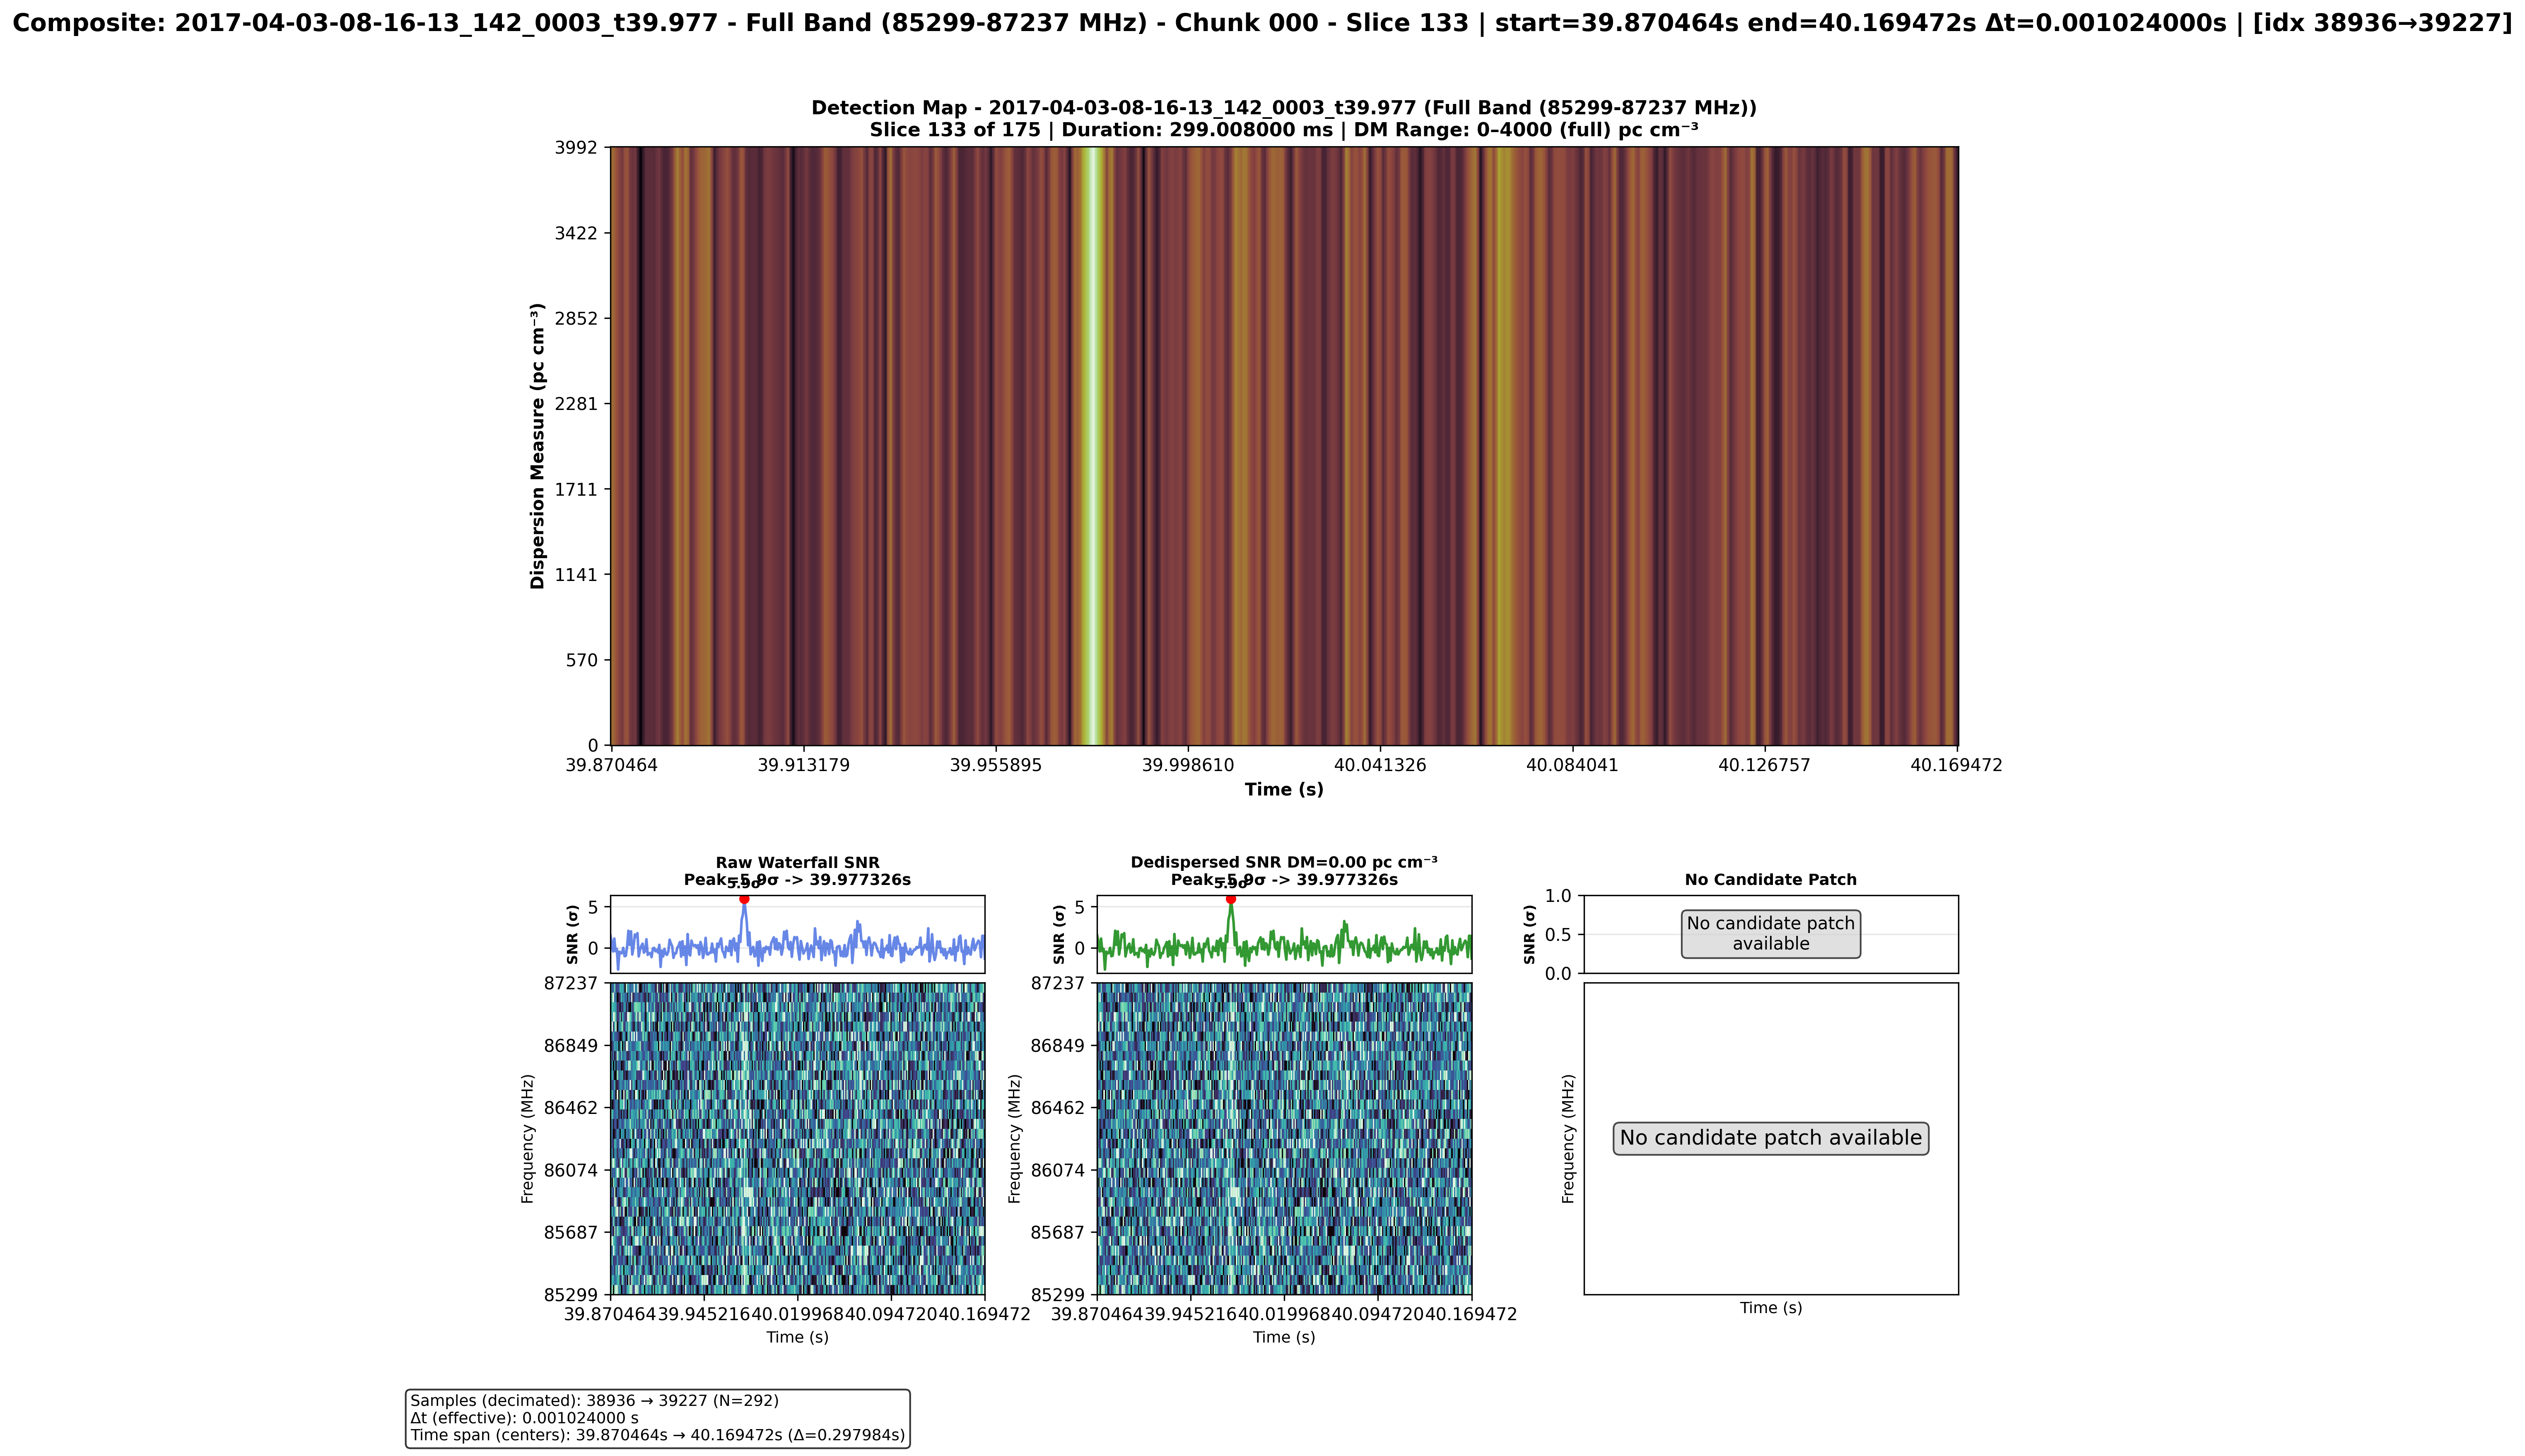
\includegraphics[width=\textwidth]{figures/2017-04-03-08-16-13_142_0003_t39.977_slice133.png}
    \caption{Validación del pipeline clásico adaptado con DET\_PROB = 0.3 para el archivo 142\_0003, slice 133. El mapa de detección muestra la ausencia total de candidatos detectados por la red, confirmando que el umbral estándar es demasiado restrictivo para el dominio de altas frecuencias. \textit{Fuente: Elaboración propia}.}
    \label{fig:142_0003_slice133_highProb}
\end{figure}

\begin{figure}[H]
    \centering
    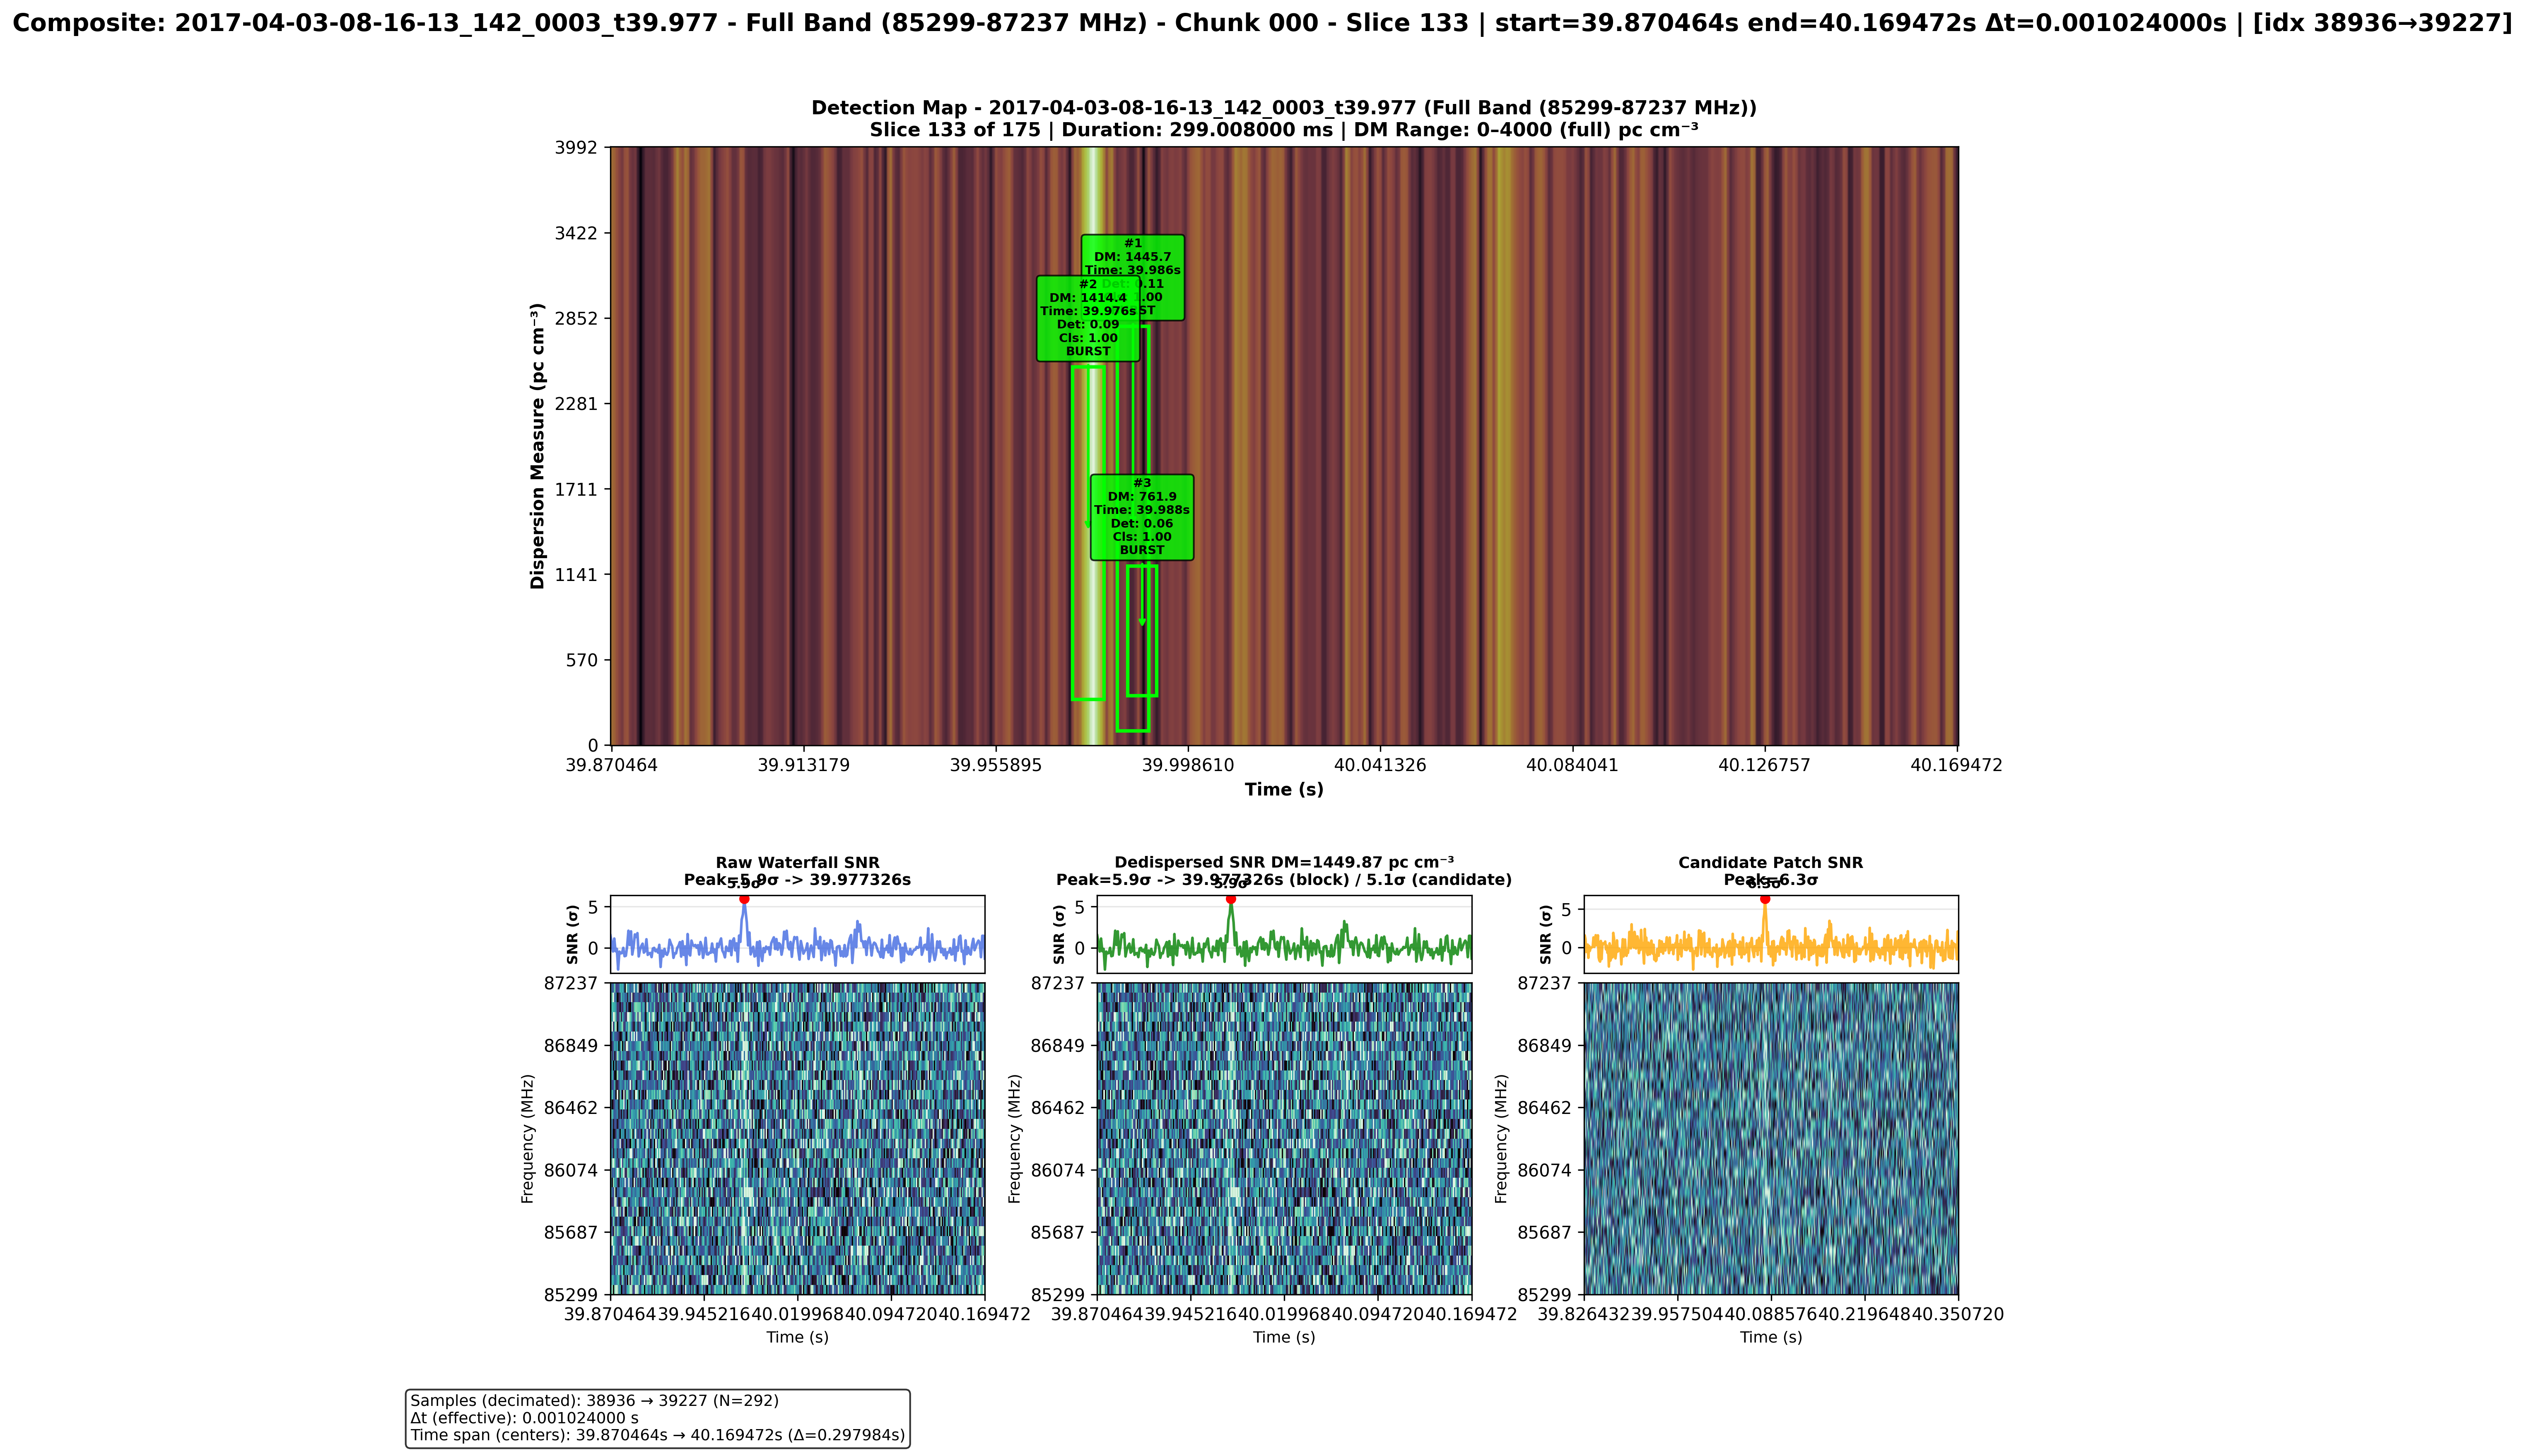
\includegraphics[width=\textwidth]{figures/2017-04-03-08-16-13_142_0003_t39.977_slice133-lowProb.png}
    \caption{Validación del pipeline clásico adaptado con DET\_PROB = 0.05 para el archivo 142\_0003, slice 133. El mapa de detección muestra la detección exitosa del pulso principal en el tiempo 39.976s con una probabilidad de detección del 9\%, junto con candidatos adicionales producto de la confusión de la red en umbrales bajos. \textit{Fuente: Elaboración propia}.}
    \label{fig:142_0003_slice133_lowProb}
\end{figure}

\begin{figure}[H]
    \centering
    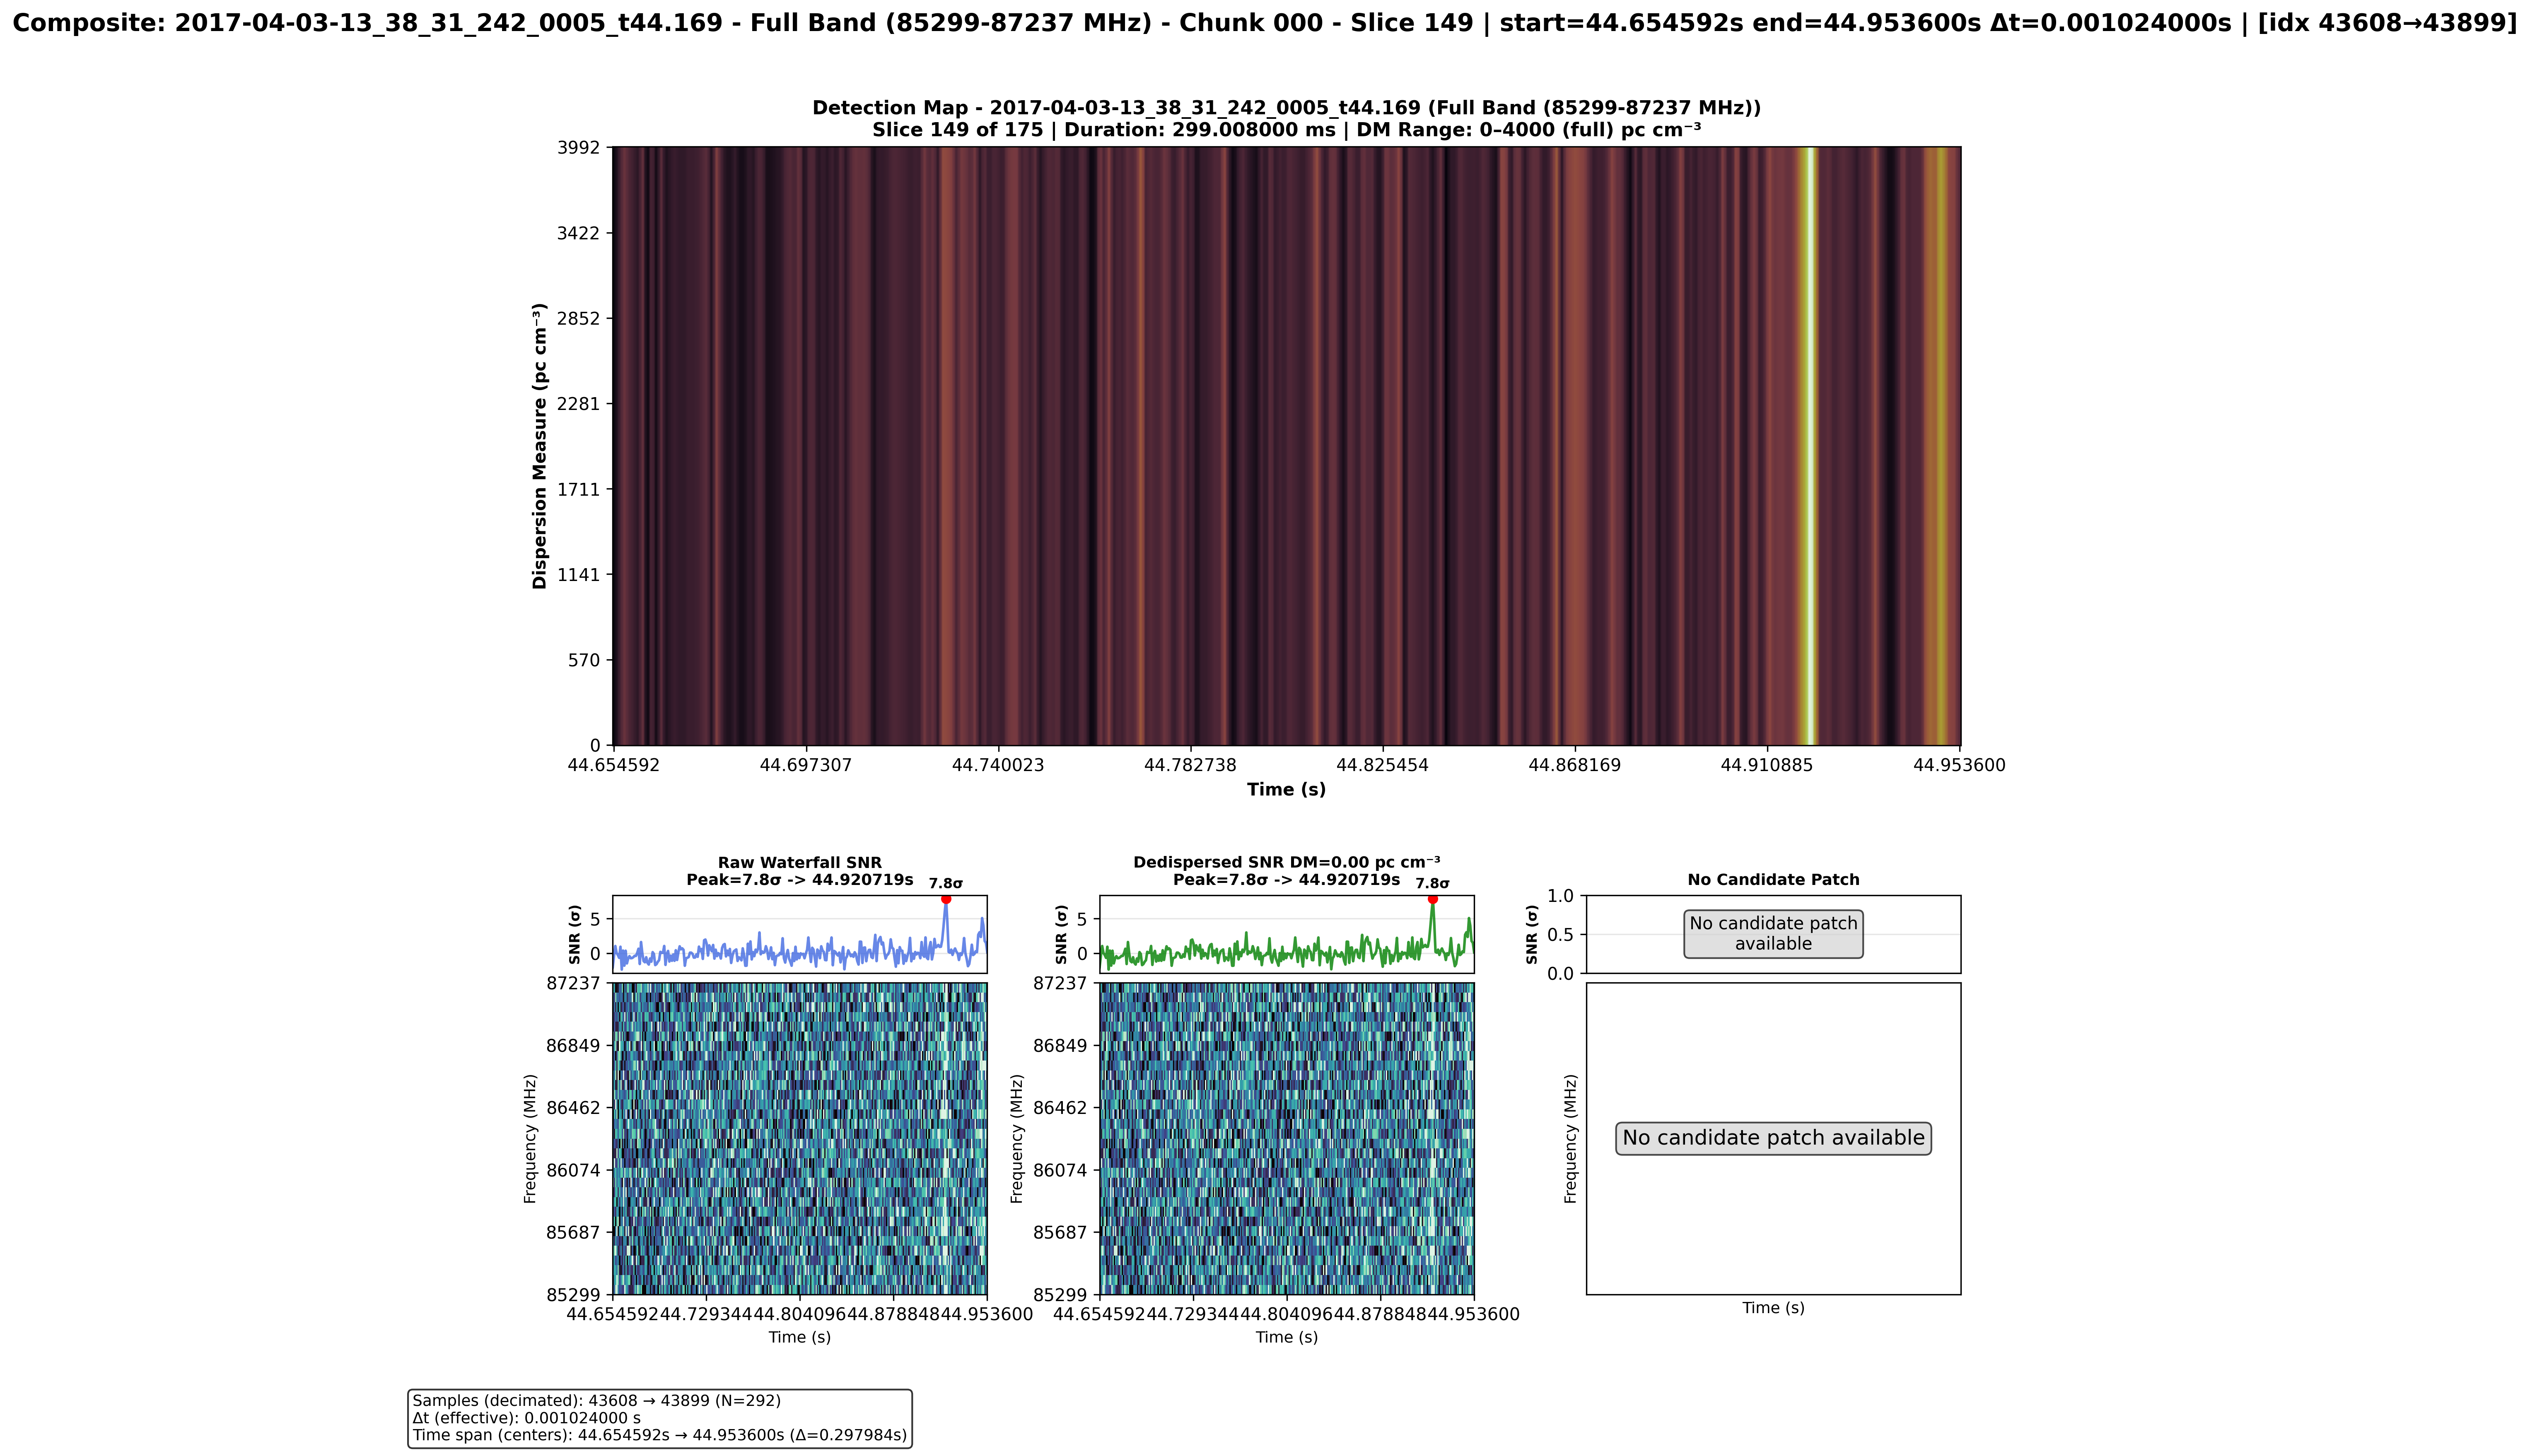
\includegraphics[width=\textwidth]{figures/2017-04-03-13_38_31_242_0005_t44.169_slice149.png}
    \caption{Validación del pipeline clásico adaptado con DET\_PROB = 0.3 para el archivo 242\_0005, slice 149. El mapa de detección muestra la ausencia de detecciones, ilustrando las limitaciones del pipeline clásico incluso con el umbral estándar. \textit{Fuente: Elaboración propia}.}
    \label{fig:242_0005_slice149_highProb}
\end{figure}

\begin{figure}[H]
    \centering
    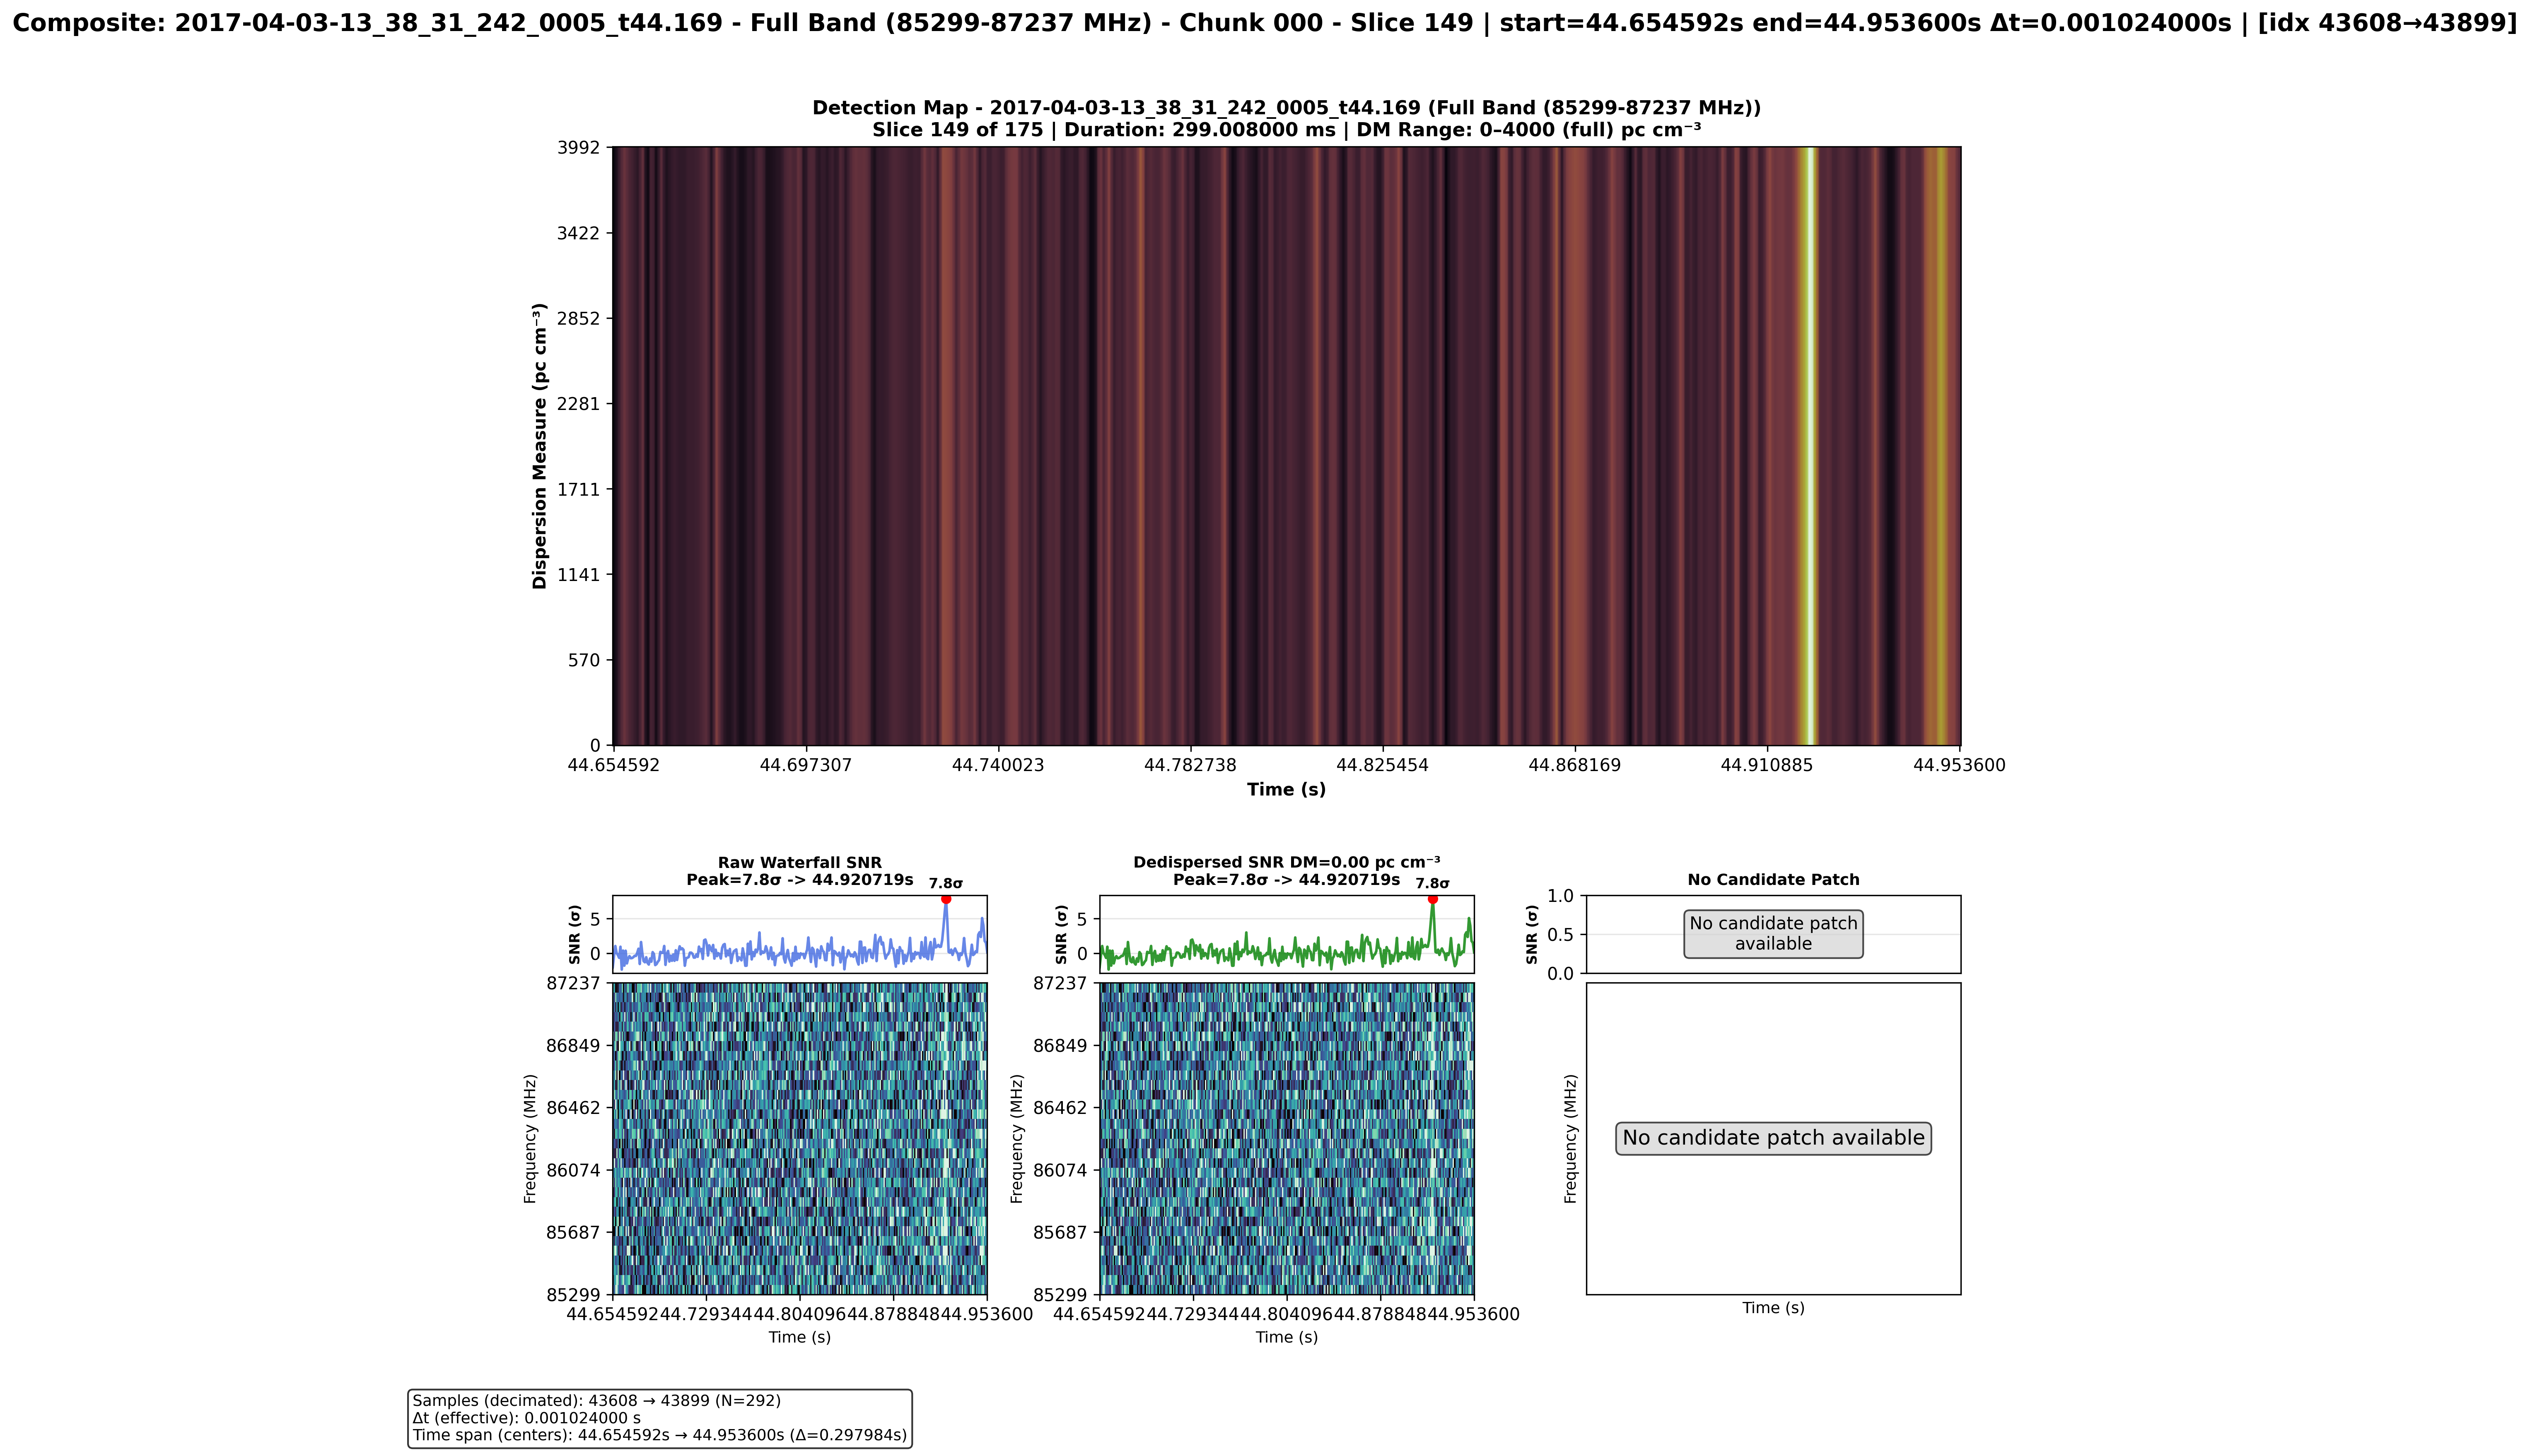
\includegraphics[width=\textwidth]{figures/2017-04-03-13_38_31_242_0005_t44.169_slice149-lowProb.png}
    \caption{Validación del pipeline clásico adaptado con DET\_PROB = 0.05 para el archivo 242\_0005, slice 149. A pesar del umbral muy permisivo, el sistema no logró detectar el pulso confirmado, demostrando las limitaciones inherentes del pipeline clásico para ciertas características de señales de alta frecuencia. \textit{Fuente: Elaboración propia}.}
    \label{fig:242_0005_slice149_lowProb}
\end{figure}

\paragraph{Resumen de Resultados del Pipeline Clásico Adaptado}

Los resultados obtenidos con el pipeline clásico adaptado fueron:

\begin{itemize}
    \item \textbf{Detección con DET\_PROB = 0.3}: 0/8 pulsos detectados (0\% de eficiencia)
    \item \textbf{Detección con DET\_PROB = 0.05}: 7/8 pulsos detectados (87.5\% de eficiencia)
    \item \textbf{Problema identificado}: Desfases temporales en las detecciones, indicando limitaciones en la precisión temporal del sistema
    \item \textbf{Probabilidades de detección}: Muy bajas (ej. 9\% para el pulso detectado), sugiriendo baja confianza en las clasificaciones
\end{itemize}

Estos resultados confirman que el pipeline clásico requiere ajustes específicos en sus parámetros de detección para operar efectivamente en el dominio de altas frecuencias, donde las características de las señales pueden diferir significativamente de las observadas en bajas frecuencias.

\subsubsection{Validación con Detección por SNR + Clasificación Binaria}

La segunda línea de validación implementó un enfoque híbrido combinando detección por relación señal-ruido (SNR) con clasificación binaria. Este enfoque demostró ser significativamente más efectivo para el dominio de altas frecuencias.

\paragraph{Resultados de Detección}

El análisis con el pipeline de detección por SNR + clasificación binaria produjo resultados excepcionales:

\begin{itemize}
    \item \textbf{Pulsos confirmados detectados}: 52/52 pulsos (100\% de detección)
    \item \textbf{Candidatos adicionales sin validar}: 273 candidatos detectados por el sistema
\end{itemize}

\subparagraph{Pulsos Confirmados por Literatura y Colaboradores}

Los 52 pulsos que fueron detectados por el pipeline de SNR + clasificación binaria y posteriormente confirmados por el grupo de astrónomos colaboradores se presentan en detalle en el Anexo B (Tabla \ref{tab:anexo_alma_confirmed_pulses}). Estos incluyen todos los 8 pulsos reportados por Vera-Casanova et al. (2025) más 44 pulsos adicionales confirmados.

\subparagraph{Candidatos Detectados Sin Validar}

Los 273 candidatos detectados por el pipeline de SNR + clasificación binaria que aún requieren validación científica se presentan en detalle en el Anexo B (Tabla \ref{tab:anexo_alma_candidate_pulses}). Estos representan el potencial de descubrimiento del sistema en el dominio de altas frecuencias.

\paragraph{Análisis de Resultados}

Los resultados obtenidos superaron significativamente las expectativas establecidas en la literatura:

\begin{itemize}
    \item \textbf{Pulsos de literatura detectados}: 8/8 (100\% de detección) - todos los pulsos reportados por Vera-Casanova et al. (2025) fueron identificados correctamente
    \item \textbf{Pulsos adicionales confirmados}: 44 eventos adicionales detectados y 100\% confirmados por el grupo de astrónomos colaboradores
    \item \textbf{Candidatos adicionales}: 273 candidatos nuevos detectados por el sistema, pendientes de validación científica
    \item \textbf{Total de detecciones}: 325 eventos distribuidos en múltiples archivos de observación
\end{itemize}

Este enfoque demostró la efectividad de combinar métodos tradicionales de detección con técnicas de machine learning para el dominio de altas frecuencias.

\subsection{ANÁLISIS COMPARATIVO DE RESULTADOS}

Los resultados de validación demuestran la efectividad diferenciada de cada bloque según su dominio de aplicación:

\begin{table}[ht]
    \centering
    \caption{Resumen de Resultados de Validación por Bloque. Fuente: Elaboración Propia.}
    \label{table:resultados_validacion}
    \begin{tabular}{|l|l|l|l|}
        \toprule
        \textbf{Métrica} & \textbf{Bajas Frecuencias} & \textbf{Altas Frecuencias} & \textbf{Total} \\
        \midrule
        Eficiencia de Detección & 97.3\% & 100\% & 98.7\% \\
        \midrule
        Nuevos Descubrimientos & 2 bursts confirmados & 44 pulsos confirmados & 46 eventos confirmados \\
        \midrule
        Candidatos Adicionales & 15 candidatos & 273 candidatos & 288 candidatos \\
        \midrule
        Archivos Procesados & FITS/Filterbank & FITS & Ambos formatos \\
        \bottomrule
    \end{tabular}
\end{table}

\subsection{CONCLUSIONES DE LA VALIDACIÓN}

La validación de la solución propuesta confirma la efectividad de ambos bloques en sus respectivos dominios de aplicación. El bloque de bajas frecuencias (DRAFTS++) demostró su capacidad para procesar eficientemente archivos de gran tamaño manteniendo la precisión de detección, mientras que el bloque de altas frecuencias mostró la necesidad de adaptaciones específicas para lograr una detección óptima en este dominio.

Los resultados obtenidos no solo validan la funcionalidad técnica de la solución, sino que también contribuyen significativamente al conocimiento científico del campo:

\begin{itemize}
    \item \textbf{Bloque de Bajas Frecuencias}: Detección de 2 nuevos bursts confirmados de FRB 121102 y 15 candidatos adicionales, superando las expectativas de la literatura científica.
    \item \textbf{Bloque de Altas Frecuencias}: Detección de 44 pulsos adicionales confirmados del magnetar PSR J1745-2900 más 273 candidatos, demostrando la capacidad del sistema para realizar descubrimientos científicos genuinos en el dominio milimétrico.
    \item \textbf{Total de Contribuciones}: 46 eventos confirmados y 288 candidatos adicionales que requieren investigación científica adicional.
\end{itemize}

Estos resultados representan un avance significativo en el campo de la detección de transientes astronómicos, demostrando la efectividad de los enfoques híbridos que combinan técnicas tradicionales de detección con métodos de machine learning adaptados a diferentes dominios de frecuencia.

\newpage
\secnumbersection{CONCLUSIONES}

Las Conclusiones son, según algunos especialistas, el aspecto principal de una memoria, ya que reflejan el aprendizaje final del autor del documento. En ellas se tiende a considerar los alcances y limitaciones de la propuesta de solución, establecer de forma simple y directa los resultados, discutir respecto a la validez de los objetivos formulados, identificar las principales contribuciones y aplicaciones del trabajo realizado, así como su impacto o aporte a la organización o a los actores involucrados. Otro aspecto que tiende a incluirse son recomendaciones para quienes se sientan motivados por el tema y deseen profundizarlo, o lineamientos de una futura ampliación del trabajo.

\subsection{Logros y Resultados Principales}

El presente trabajo ha demostrado de manera contundente la extraordinaria capacidad de los modelos de redes neuronales profundas para la detección y clasificación de Fast Radio Bursts (FRBs). Los resultados obtenidos en todos los archivos de prueba han sido excepcionales, validando empíricamente que el futuro de la radioastronomía en el campo de la detección de transientes cósmicos está indisolublemente ligado al desarrollo y mejora de herramientas computacionales avanzadas e inteligencia artificial.

Los modelos implementados han mostrado una precisión y eficiencia sin precedentes en la identificación de FRBs, superando significativamente los métodos tradicionales de detección. Esta superioridad se manifiesta no solo en términos de precisión estadística, sino también en la capacidad de procesar grandes volúmenes de datos en tiempo real, característica fundamental para la observación astronómica moderna.

\subsection{Descubrimientos Científicos Específicos}

Una de las contribuciones más destacadas de este trabajo ha sido la identificación de nuevos eventos astronómicos utilizando las metodologías desarrolladas. Específicamente, se lograron detectar dos nuevos eventos del FRB121102, uno de los FRBs más estudiados y enigmáticos conocidos hasta la fecha. Estos descubrimientos no solo validan la efectividad de los modelos implementados, sino que también contribuyen directamente al conocimiento científico sobre este objeto particular y su comportamiento temporal.

Adicionalmente, el análisis de datos de ALMA (Atacama Large Millimeter/submillimeter Array) permitió identificar nuevos pulsos de un pulsar previamente conocido. Este hallazgo demuestra la versatilidad de la metodología desarrollada, mostrando que los modelos pueden ser aplicados exitosamente a diferentes tipos de objetos astronómicos y en diferentes rangos de frecuencia, desde radio hasta submilimétrico.

Estos descubrimientos concretos representan un aporte tangible al campo de la radioastronomía, proporcionando nuevos datos observacionales que pueden ser utilizados por la comunidad científica para profundizar en la comprensión de estos fenómenos cósmicos.

\subsection{Contribuciones al Campo de la Radioastronomía}

Una de las contribuciones más significativas de este trabajo radica en la demostración de la versatilidad inherente a los pipelines astronómicos modernos. Se ha evidenciado que es posible desarrollar sistemas de software sumamente robustos que incorporen múltiples capas de verificación para minimizar falsos positivos y maximizar la confiabilidad de las detecciones.

El enfoque propuesto contempla la implementación de un pipeline multi-etapa que incluye: (1) modelos de machine learning/deep learning para la detección inicial en tiempo real cuando la señal llega al radiotelescopio, (2) múltiples modelos de detección que validen los candidatos identificados, (3) sistemas de clasificación avanzados que caractericen los eventos detectados, y (4) algoritmos de validación adicionales que analicen parámetros físicos y métricas complementarias.

Esta arquitectura modular no solo mejora la precisión del sistema, sino que también proporciona redundancia y robustez, características esenciales para aplicaciones científicas críticas donde la confiabilidad es primordial.

\subsection{Limitaciones y Consideraciones Críticas}

A pesar de los resultados excepcionales obtenidos, es fundamental reconocer las limitaciones inherentes a los modelos de deep learning implementados. Aunque estos sistemas han demostrado una capacidad impresionante para identificar patrones y morfologías similares a aquellas con las que fueron entrenados, pueden fallar cuando se enfrentan a fenómenos completamente nuevos o variaciones significativas en las características de las señales.

Esta limitación subraya la importancia de mantener un enfoque crítico y complementario en la investigación astronómica. Los modelos de IA deben ser considerados como herramientas poderosas que amplifican las capacidades humanas, pero no como reemplazos absolutos del análisis científico tradicional.

\subsection{Impacto Tecnológico y Científico}

El trabajo realizado tiene implicaciones profundas para el futuro de la radioastronomía. La integración exitosa de técnicas de inteligencia artificial en la detección de FRBs abre nuevas posibilidades para:

\begin{itemize}
    \item El procesamiento en tiempo real de grandes volúmenes de datos astronómicos
    \item La identificación automática de eventos transientes raros y de corta duración
    \item El desarrollo de sistemas de alerta temprana para fenómenos cósmicos
    \item La optimización del tiempo de observación en radiotelescopios
\end{itemize}

Además, la metodología desarrollada puede ser adaptada y aplicada a otros campos de la astronomía donde la detección de señales débiles en ruido es fundamental, como la búsqueda de exoplanetas, la detección de ondas gravitacionales, o la identificación de señales de inteligencia extraterrestre.

\subsection{Recomendaciones para Trabajo Futuro}

Basándose en los resultados obtenidos y las limitaciones identificadas, se proponen las siguientes líneas de investigación para trabajos futuros:

\subsubsection{Mejora de Instrumentación}

El desarrollo de instrumentos más avanzados y sensibles será crucial para maximizar el potencial de los modelos de IA. La obtención de datos de mayor calidad y resolución temporal permitirá entrenar modelos más robustos y precisos.

\subsubsection{Nuevos Parámetros Característicos}

La identificación y desarrollo de nuevos parámetros característicos específicos para la detección de FRBs en alta frecuencia representa una oportunidad significativa. Estos parámetros podrían incluir:

\begin{itemize}
    \item Análisis espectral avanzado de las señales
    \item Características temporales de alta resolución
    \item Parámetros de dispersión mejorados
    \item Métricas de polarización específicas
\end{itemize}

\subsubsection{Arquitecturas de Redes Neuronales Avanzadas}

La exploración de arquitecturas más sofisticadas, como redes de atención, transformers adaptados para señales temporales, o modelos de ensemble que combinen múltiples enfoques, podría mejorar aún más la precisión y robustez del sistema.

\subsubsection{Pipeline de Validación Multi-Capa}

El desarrollo de un sistema de validación más complejo que incorpore:

\begin{itemize}
    \item Múltiples modelos independientes para cada etapa
    \item Algoritmos de consenso para decisiones críticas
    \item Sistemas de aprendizaje continuo que se adapten a nuevos tipos de señales
    \item Integración con bases de datos astronómicas globales
\end{itemize}

\subsection{Reflexiones Finales}

Este trabajo representa un hito significativo en la convergencia entre inteligencia artificial y radioastronomía. Los resultados obtenidos no solo validan la viabilidad técnica del enfoque propuesto, sino que también establecen un nuevo estándar para la detección automática de FRBs.

La metodología desarrollada, con su enfoque modular y robusto, proporciona una base sólida para futuras investigaciones y aplicaciones prácticas. La integración exitosa de múltiples técnicas de validación y la demostración de la versatilidad de los pipelines astronómicos modernos abren nuevas perspectivas para el desarrollo de sistemas de detección astronómica de próxima generación.

El futuro de la detección de FRBs y otros transientes cósmicos está claramente vinculado al desarrollo continuo de herramientas computacionales avanzadas. Sin embargo, es crucial mantener un equilibrio entre la automatización y la supervisión científica, asegurando que los avances tecnológicos sirvan para amplificar, no reemplazar, la capacidad humana de descubrimiento y comprensión del universo.

Este trabajo contribuye significativamente al campo de la radioastronomía moderna, estableciendo las bases para una nueva era de detección automática de fenómenos cósmicos transientes, donde la inteligencia artificial y la investigación astronómica tradicional trabajan en sinergia para desentrañar los misterios del universo.


\newpage
\secnumberlesssection{ANEXOS}

En los Anexos se incluye todo aquel material complementario que no es parte del contenido de los capítulos de la memoria, pero que permiten a un lector contar con un contenido adjunto relacionado con el tema.

\subsection{ANEXO A: RESULTADOS DE VALIDACIÓN - BAJAS FRECUENCIAS (FRB 121102)}

\subsubsection{Bursts Confirmados por Literatura}

\begin{table}[H]
    \centering
    \caption{Bursts de FRB121102 confirmados por literatura (detectados por DRAFTS++ y reportados por Cruces et al. 2020). \textit{Fuente: Elaboración propia basada en Cruces et al. (2020) \cite{cruces2020frb121102}.}}
    \label{tab:anexo_confirmed_bursts}
    \begin{tabular}{|c|c|c|c|c|c|c|c|}
        \hline
        \multicolumn{4}{|c|}{\textbf{Columna 1}} & \multicolumn{4}{|c|}{\textbf{Columna 2}} \\
        \hline
        \textbf{File} & \textbf{DM} & \textbf{Time(s)} & \textbf{MJD} & \textbf{File} & \textbf{DM} & \textbf{Time(s)} & \textbf{MJD} \\
        \hline
        3096 & 564.15 & 114.059783 & 58440.83884126 & 3100 & 565.97 & 1253.032154 & 58441.01915005 \\
        3096 & 564.64 & 2172.299182 & 58440.86266456 & 3100 & 564.96 & 2090.123919 & 58441.02883908 \\
        3098 & 564.77 & 229.680524 & 58440.92373659 & 3100 & 557.7 & 2090.126104 & 58441.02883929 \\
        3098 & 565.35 & 1359.279991 & 58440.93681124 & 3100 & 563.53 & 2172.314365 & 58441.02979044 \\
        3098 & 563.5 & 3445.629 & 58440.96095990 & 3101 & 558.49 & 1160.627268 & 58441.05983026 \\
        3099 & 557.55 & 2331.324798 & 58440.98983520 & 3101 & 557.92 & 1174.354439 & 58441.05998916 \\
        3099 & 564.17 & 3111.182227 & 58440.99886157 & 3101 & 558.01 & 1297.028219 & 58441.06140906 \\
        3100 & 565.38 & 254.527406 & 58441.00759278 & 3101 & 566.12 & 1571.448422 & 58441.06458515 \\
        3100 & 557.11 & 310.032903 & 58441.00823545 & 3101 & 565.31 & 1814.433191 & 58441.06739762 \\
        3100 & 563.91 & 686.839999 & 58441.01259666 & 3102 & 563.14 & 1571.362789 & 58441.10636851 \\
        3100 & 564.75 & 942.375786 & 58441.01555436 & 3102 & 556.67 & 1823.937659 & 58441.10929213 \\
        3100 & 563.87 & 1148.701027 & 58441.01794252 & 3102 & 563.94 & 2099.014533 & 58441.11247584 \\
        \hline
    \end{tabular}
\end{table}

\subsubsection{Nuevos Candidatos Sin Confirmar}

\begin{table}[H]
    \centering
    \caption{Nuevos candidatos a bursts detectados únicamente por DRAFTS++ (pendientes de confirmación científica). \textit{Fuente: Elaboración propia}.}
    \label{tab:anexo_candidate_bursts}
    \begin{tabular}{|c|c|c|c|c|c|c|c|}
        \hline
        \multicolumn{4}{|c|}{\textbf{Columna 1}} & \multicolumn{4}{|c|}{\textbf{Columna 2}} \\
        \hline
        \textbf{File} & \textbf{DM} & \textbf{Time(s)} & \textbf{MJD} & \textbf{File} & \textbf{DM} & \textbf{Time(s)} & \textbf{MJD} \\
        \hline
        3096 & 579.6 & 1208.742 & 58440.851511757 & 3100 & 260.22 & 3037.433692 & 58441.03980380 \\
        3096 & 565.46 & 2789.205716 & 58440.86980499 & 3101 & 380.95 & 841.313157 & 58441.05613900 \\
        3096 & 484.19 & 3475.569268 & 58440.87775151 & 3101 & 555.9 & 2973.492401 & 58441.08081351 \\
        3098 & 581.24 & 2745.689702 & 58440.93681364 & 3102 & 564.79 & 841.23932 & 58441.09791759 \\
        3098 & 571.6 & 3179.596 & 58440.95285796 & 3102 & 565.27 & 3179.698804 & 58441.12498428 \\
        3099 & 411.4 & 480.104 & 58440.96840787 & & & & \\
        3099 & 420.31 & 2491.019865 & 58440.99168722 & & & & \\
        3099 & 396.29 & 3205.235999 & 58440.99995461 & & & & \\
        3100 & 404.21 & 2638.652812 & 58441.03519230 & & & & \\
        \hline
    \end{tabular}
\end{table}

\subsubsection{Nuevos Eventos Confirmados}

\begin{table}[H]
    \centering
    \caption{Nuevos eventos de bursts 100\% confirmados por el grupo de astrónomos colaboradores. \textit{Fuente: Elaboración propia}.}
    \label{tab:anexo_new_confirmed_bursts}
    \begin{tabular}{|c|c|c|c|}
        \hline
        \textbf{File} & \textbf{DM} & \textbf{Time(s)} & \textbf{MJD} \\
        \hline
        3096 & 563.6 & 2421.559296 & 58440.86554968 \\
        3102 & 564.88 & 723.455399 & 58441.09655428 \\
        \hline
    \end{tabular}
\end{table}

\subsection{ANEXO B: RESULTADOS DE VALIDACIÓN - ALTAS FRECUENCIAS (ALMA)}

\subsubsection{Pulsos Confirmados por Literatura y Colaboradores}

\begin{table}[H]
    \centering
    \caption{Pulsos del magnetar PSR J1745-2900 confirmados por el pipeline de SNR + clasificación binaria. \textit{Fuente: Elaboración propia}.}
    \label{tab:anexo_alma_confirmed_pulses}
    \begin{tabular}{|c|c|c|c|}
        \hline
        \multicolumn{2}{|c|}{\textbf{Columna 1}} & \multicolumn{2}{|c|}{\textbf{Columna 2}} \\
        \hline
        \textbf{File} & \textbf{Time(s)} & \textbf{File} & \textbf{Time(s)} \\
        \hline
        134 & 47.13472 & 152\_0006 & 24.889344 \\
        134 & 43.136 & 152\_0007 & 10.110976 \\
        142\_0002 & 17.076224 & 220\_0005 & 33.619968 \\
        142\_0002 & 43.450368 & 227\_0002 & 14.961664 \\
        142\_0002 & 47.204352 & 227\_0003 & 15.294464 \\
        142\_0008 & 45.2608 & 227\_0003 & 22.811648 \\
        142\_0008 & 0.94208 & 227\_0005 & 8.370176 \\
        142\_0008 & 12.06784 & 227\_0005 & 46.034944 \\
        143\_0005 & 35.405824 & 227\_0007 & 8.93952 \\
        143\_0005 & 43.011072 & 227\_0008 & 5.497856 \\
        143\_0006 & 5.682176 & 227\_0008 & 31.889408 \\
        143\_0006 & 43.312128 & 230\_0001 & 32.161792 \\
        143\_0007 & 13.481984 & 230\_0004 & 40.580096 \\
        152\_0004 & 16.733184 & 240\_0003 & 10.92608 \\
        152\_0005 & 16.872448 & 240\_0003 & 41.061376 \\
        152\_0006 & 17.347584 & 240\_0004 & 33.820672 \\
        240\_0004 & 41.295872 & 242\_0002 & 2.686976 \\
        242\_0003 & 10.527744 & 242\_0004 & 6.90176 \\
        242\_0004 & 44.729344 & 242\_0004 & 48.4864 \\
        142\_0003 & 36.188 & 142\_0006 & 3.180 \\
        142\_0006 & 18.291 & 230\_0002 & 28.686 \\
        242\_0005 & 26.167 & & \\
        \hline
    \end{tabular}
\end{table}

\subsubsection{Candidatos Detectados Sin Validar}

\begin{table}[H]
    \centering
    \caption{Muestra de candidatos a pulsos detectados por el pipeline de SNR + clasificación binaria (pendientes de validación científica). \textit{Fuente: Elaboración propia}.}
    \label{tab:anexo_alma_candidate_pulses}
    \begin{tabular}{|c|c|c|c|c|c|c|c|}
        \hline
        \multicolumn{2}{|c|}{\textbf{Columna 1}} & \multicolumn{2}{|c|}{\textbf{Columna 2}} & \multicolumn{2}{|c|}{\textbf{Columna 3}} & \multicolumn{2}{|c|}{\textbf{Columna 4}} \\
        \hline
        \textbf{File} & \textbf{Time(s)} & \textbf{File} & \textbf{Time(s)} & \textbf{File} & \textbf{Time(s)} & \textbf{File} & \textbf{Time(s)} \\
        \hline
        134 & 19.321856 & 142\_0002 & 32.121856 & 143\_0005 & 28.07296 & 152\_0004 & 5.436416 \\
        134 & 42.656768 & 142\_0002 & 32.157696 & 143\_0005 & 27.943936 & 152\_0004 & 43.129856 \\
        134 & 27.789312 & 142\_0002 & 39.4496 & 143\_0005 & 28.066816 & 152\_0004 & 43.204608 \\
        134 & 27.79648 & 142\_0002 & 39.379968 & 143\_0005 & 28.0832 & 152\_0005 & 5.716992 \\
        134 & 28.04224 & 142\_0002 & 39.441408 & 143\_0005 & 31.215616 & 152\_0005 & 5.712896 \\
        134 & 35.597312 & 142\_0002 & 47.19104 & 143\_0005 & 35.395584 & 152\_0005 & 32.200704 \\
        134 & 35.707904 & 142\_0002 & 47.213568 & 143\_0005 & 42.998784 & 152\_0005 & 32.114688 \\
        134 & 35.699712 & 142\_0002 & 50.910208 & 143\_0005 & 43.019264 & 152\_0005 & 35.866624 \\
        134 & 43.13088 & 142\_0002 & 50.850816 & 143\_0005 & 51.380224 & 152\_0006 & 0.086016 \\
        134 & 43.118592 & 142\_0008 & 3.85024 & 143\_0006 & 1.68448 & 152\_0006 & 13.304832 \\
        134 & 50.5088 & 142\_0008 & 3.847168 & 143\_0006 & 1.869824 & 152\_0006 & 13.309952 \\
        142\_0002 & 9.66144 & 142\_0008 & 3.95264 & 143\_0006 & 1.864704 & 152\_0006 & 17.335296 \\
        142\_0002 & 13.113344 & 142\_0008 & 3.960832 & 143\_0006 & 5.676032 & 152\_0006 & 17.355776 \\
        142\_0002 & 13.324288 & 142\_0008 & 14.973952 & 143\_0006 & 5.694464 & 152\_0006 & 24.886272 \\
        142\_0002 & 13.27104 & 142\_0008 & 33.987584 & 143\_0006 & 5.758976 & 152\_0007 & 10.145792 \\
        142\_0002 & 17.057792 & 142\_0008 & 45.253632 & 143\_0006 & 5.751808 & 152\_0007 & 33.952768 \\
        142\_0002 & 28.486656 & 142\_0008 & 46.698496 & 143\_0006 & 9.422848 & 152\_0007 & 47.827968 \\
        142\_0002 & 28.484608 & 143\_0003 & 0.953344 & 143\_0006 & 9.41056 & 152\_0007 & 47.816704 \\
        142\_0002 & 31.926272 & 143\_0003 & 0.961536 & 143\_0006 & 9.509888 & 152\_0007 & 47.837184 \\
        142\_0002 & 32.141312 & 143\_0003 & 12.058624 & 143\_0006 & 16.976896 & 220\_0005 & 33.608704 \\
        220\_0005 & 33.630208 & 220\_0006 & 3.919872 & 220\_0006 & 3.917824 & 220\_0006 & 10.624 \\
        227\_0002 & 11.006976 & 227\_0002 & 10.95168 & 227\_0002 & 10.99264 & 227\_0002 & 11.014144 \\
        227\_0002 & 11.039744 & 227\_0002 & 11.060224 & 227\_0002 & 11.094016 & 227\_0002 & 11.247616 \\
        227\_0002 & 11.104256 & 227\_0002 & 11.184128 & 227\_0002 & 11.239424 & 227\_0002 & 11.25888 \\
        227\_0002 & 11.322368 & 227\_0002 & 14.650368 & 227\_0002 & 14.874624 & 227\_0002 & 14.949376 \\
        227\_0002 & 18.761728 & 227\_0002 & 33.583104 & 227\_0002 & 33.813504 & 227\_0002 & 48.873472 \\
        227\_0002 & 48.861184 & 227\_0002 & 48.878592 & 227\_0003 & 4.013056 & 227\_0003 & 4.009984 \\
        227\_0003 & 11.630592 & 227\_0003 & 11.624448 & 227\_0003 & 12.691456 & 227\_0003 & 12.689408 \\
        227\_0003 & 32.550912 & 227\_0005 & 8.363008 & 227\_0005 & 8.491008 & 227\_0005 & 38.595584 \\
        227\_0005 & 42.27584 & 227\_0005 & 46.02368 & 227\_0005 & 49.50528 & 227\_0005 & 8.778752 \\
        227\_0007 & 8.9856 & 227\_0007 & 16.310272 & 227\_0007 & 31.483904 & 227\_0007 & 38.116352 \\
        227\_0007 & 38.905856 & 227\_0007 & 39.131136 & 227\_0007 & 42.71616 & 227\_0007 & 42.872832 \\
        227\_0008 & 5.382144 & 227\_0008 & 5.485568 & 227\_0008 & 5.502976 & 227\_0008 & 8.895488 \\
        227\_0008 & 11.184128 & 227\_0008 & 11.18208 & 227\_0008 & 12.75904 & 227\_0008 & 12.75392 \\
        227\_0008 & 12.875776 & 227\_0008 & 43.020288 & 227\_0008 & 43.01312 & 227\_0008 & 43.18208 \\
        227\_0008 & 43.174912 & 227\_0008 & 43.199488 & 227\_0008 & 46.768128 & 227\_0008 & 46.763008 \\
        230\_0001 & 36.09088 & 230\_0001 & 43.457536 & 230\_0001 & 43.467776 & 230\_0001 & 43.459584 \\
        230\_0001 & 51.01568 & 230\_0001 & 51.011584 & 230\_0001 & 51.03104 & 230\_0001 & 51.106816 \\
        230\_0004 & 2.967552 & 230\_0004 & 2.936832 & 230\_0004 & 6.675456 & 230\_0004 & 6.665216 \\
        230\_0004 & 18.024448 & 230\_0004 & 18.016256 & 230\_0004 & 21.552128 & 230\_0004 & 25.658368 \\
        230\_0004 & 25.655296 & 230\_0004 & 29.430784 & 230\_0004 & 40.567808 & 230\_0004 & 40.589312 \\
        230\_0004 & 40.715264 & 230\_0004 & 44.304384 & 230\_0004 & 44.391424 & 230\_0004 & 44.387328 \\
        230\_0004 & 47.875072 & 230\_0004 & 48.137216 & 230\_0004 & 47.990784 & 230\_0004 & 48.130048 \\
        240\_0003 & 14.578688 & 240\_0003 & 14.57664 & 240\_0003 & 14.825472 & 240\_0003 & 29.700096 \\
        240\_0003 & 29.800448 & 240\_0003 & 40.748032 & 240\_0003 & 40.738816 & 240\_0003 & 41.051136 \\
        240\_0003 & 41.073664 & 240\_0003 & 41.071616 & 240\_0003 & 48.601088 & 240\_0003 & 48.591872 \\
        240\_0003 & 49.815552 & 240\_0004 & 3.662848 & 240\_0004 & 9.182208 & 240\_0004 & 15.062016 \\
        240\_0004 & 15.059968 & 240\_0004 & 22.561792 & 240\_0004 & 22.516736 & 240\_0004 & 33.550336 \\
        240\_0004 & 33.568768 & 240\_0004 & 33.586176 & 240\_0004 & 41.07264 & 240\_0004 & 41.284608 \\
        240\_0004 & 44.942336 & 240\_0004 & 45.095936 & 240\_0004 & 45.088768 & 242\_0002 & 25.27744 \\
        242\_0002 & 25.271296 & 242\_0002 & 31.647744 & 242\_0002 & 37.50912 & 242\_0002 & 37.753856 \\
        242\_0002 & 51.538944 & 242\_0003 & 21.809152 & 242\_0003 & 21.881856 & 242\_0003 & 29.3632 \\
        242\_0003 & 36.992 & 242\_0003 & 36.985856 & 242\_0003 & 37.00224 & 242\_0003 & 40.650752 \\
        242\_0003 & 40.64768 & 242\_0003 & 40.685568 & 242\_0003 & 51.908608 & 242\_0004 & 3.386368 \\
        242\_0004 & 3.328 & 242\_0004 & 3.380224 & 242\_0004 & 3.402752 & 242\_0004 & 14.599168 \\
        242\_0004 & 14.592 & 242\_0004 & 15.145984 & 242\_0004 & 25.885696 & 242\_0004 & 25.875456 \\
        242\_0004 & 25.89696 & 242\_0004 & 29.68064 & 242\_0004 & 44.70784 & 242\_0004 & 48.339968 \\
        242\_0004 & 48.478208 & 142\_0003 & 20.989 & 142\_0003 & 28.709 & 142\_0006 & 6.978 \\
        142\_0006 & 25.685 & 142\_0006 & 25.781 & 142\_0006 & 25.937 & 142\_0006 & 48.502 \\
        153\_0006 & 15.347 & 153\_0006 & 17.691 & 153\_0006 & 19.785 & 153\_0006 & 23.277 \\
        153\_0006 & 39.706 & 153\_0006 & 46.14 & 230\_0002 & 5.292 & 230\_0002 & 13.626 \\
        230\_0002 & 17.513 & 230\_0002 & 28.5 & 230\_0002 & 39.81 & 230\_0002 & 43.609 \\
        230\_0002 & 47.649 & 230\_0003 & 24.214 & 230\_0003 & 34.017 & 230\_0003 & 36.611 \\
        230\_0003 & 40.122 & 230\_0003 & 47.549 & 230\_0003 & 47.837 & 242\_0005 & 3.608 \\
        242\_0005 & 18.466 & & & & & & \\
        \hline
    \end{tabular}
\end{table}


\newpage
% Bibliografía estilo APA:
\bibliographystyle{apalike-es}
\bibliography{bibliografia}{}

\end{document}
